\section{Efficiency}

The efficiency of each event selection is defined here in terms of the migration of events from one true topology to several reconstructed topologies.  In the case of no threshold, every topology can be reconstructed correctly and the efficiency is 100\%.  

\subsection{FHC}

\subsubsection{CC0Pi}

True CC0Pi events are always reconstructed as CC0Pi events.

\begin{center}

\includegraphics[width=0.245\textwidth]{plots/efficiency/CC0Pi_FHC_No_Threshold.pdf}
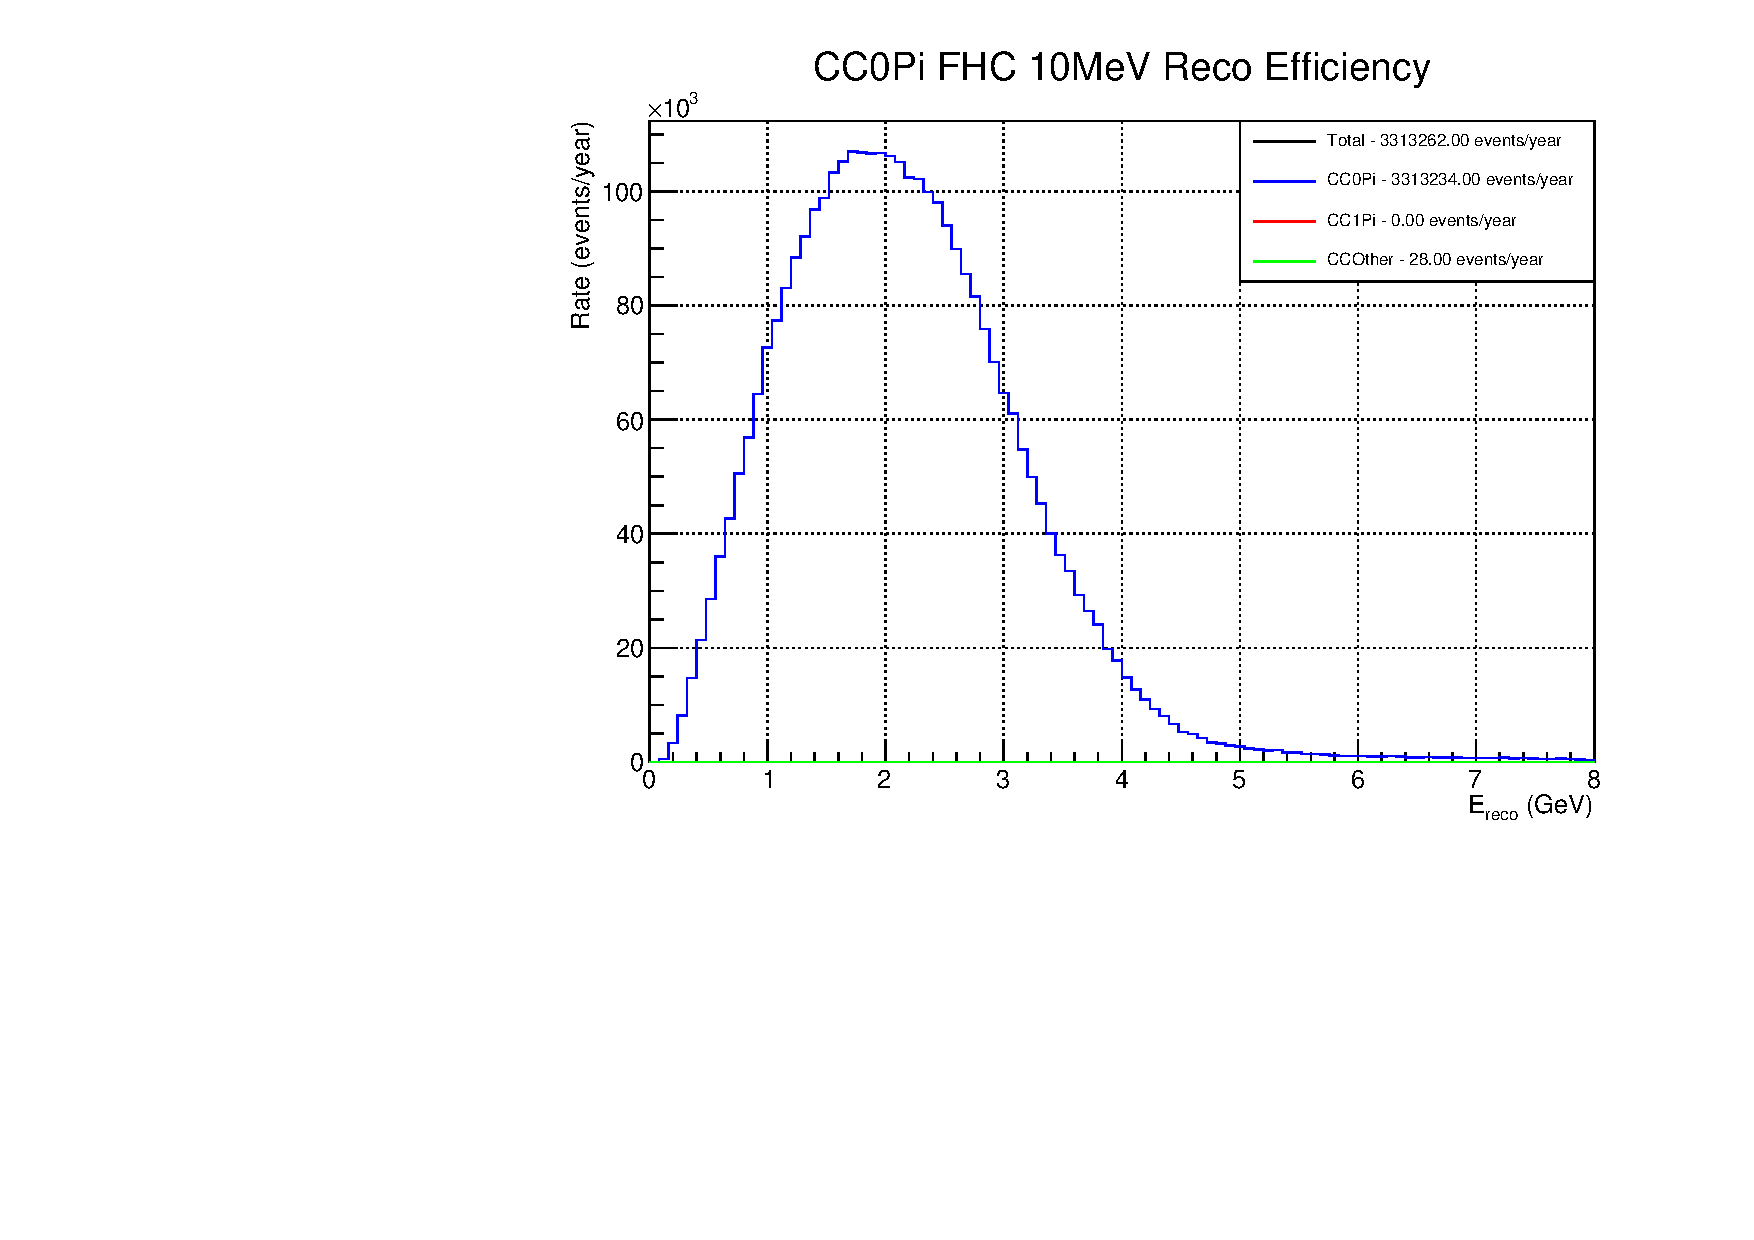
\includegraphics[width=0.245\textwidth]{plots/efficiency/CC0Pi_FHC_10MeV.pdf} 
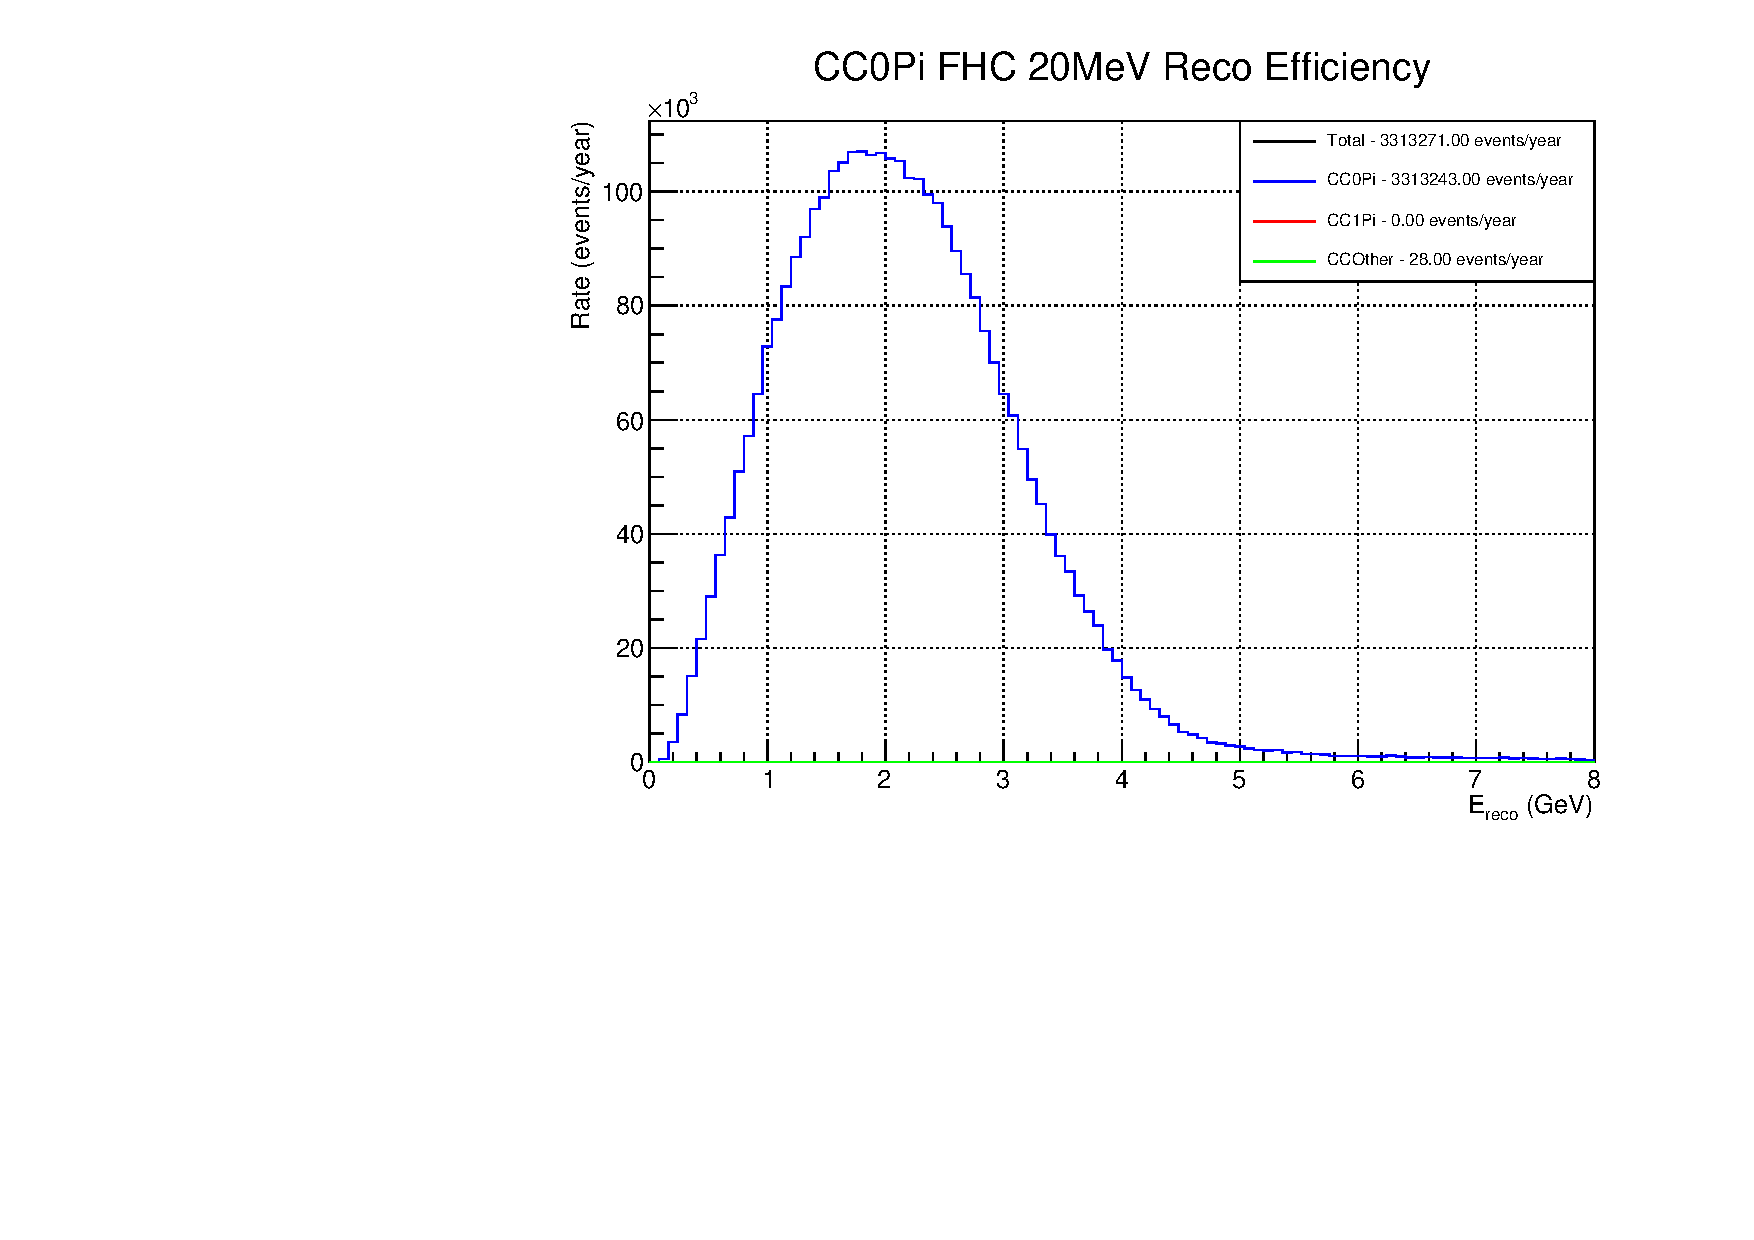
\includegraphics[width=0.245\textwidth]{plots/efficiency/CC0Pi_FHC_20MeV.pdf}
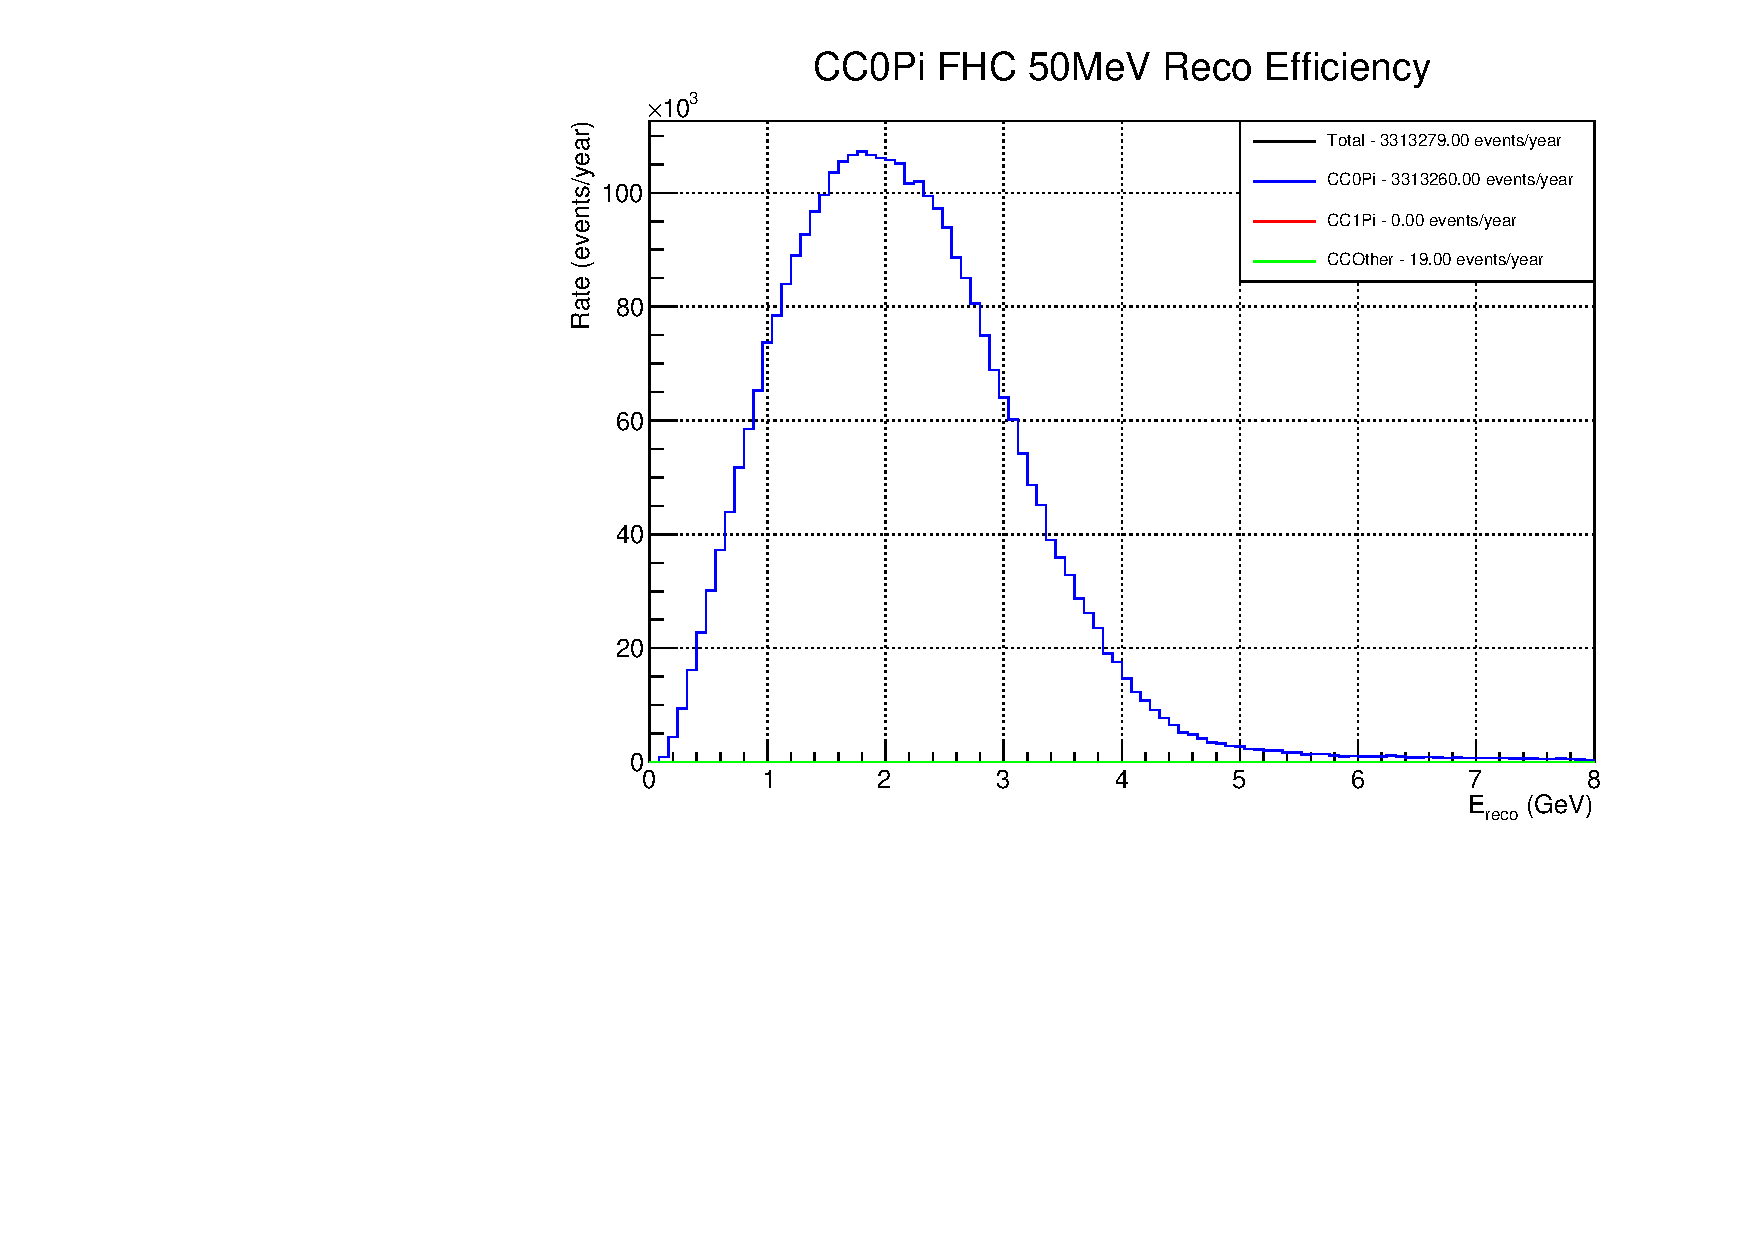
\includegraphics[width=0.245\textwidth]{plots/efficiency/CC0Pi_FHC_50MeV.pdf}

\end{center}

\subsubsection{CC1Pi}

True CC1Pi events will be reconstructed as CC0Pi events if the pion is beneath the threshold.

\begin{center}

\includegraphics[width=0.245\textwidth]{plots/efficiency/CC1Pi_FHC_No_Threshold.pdf}
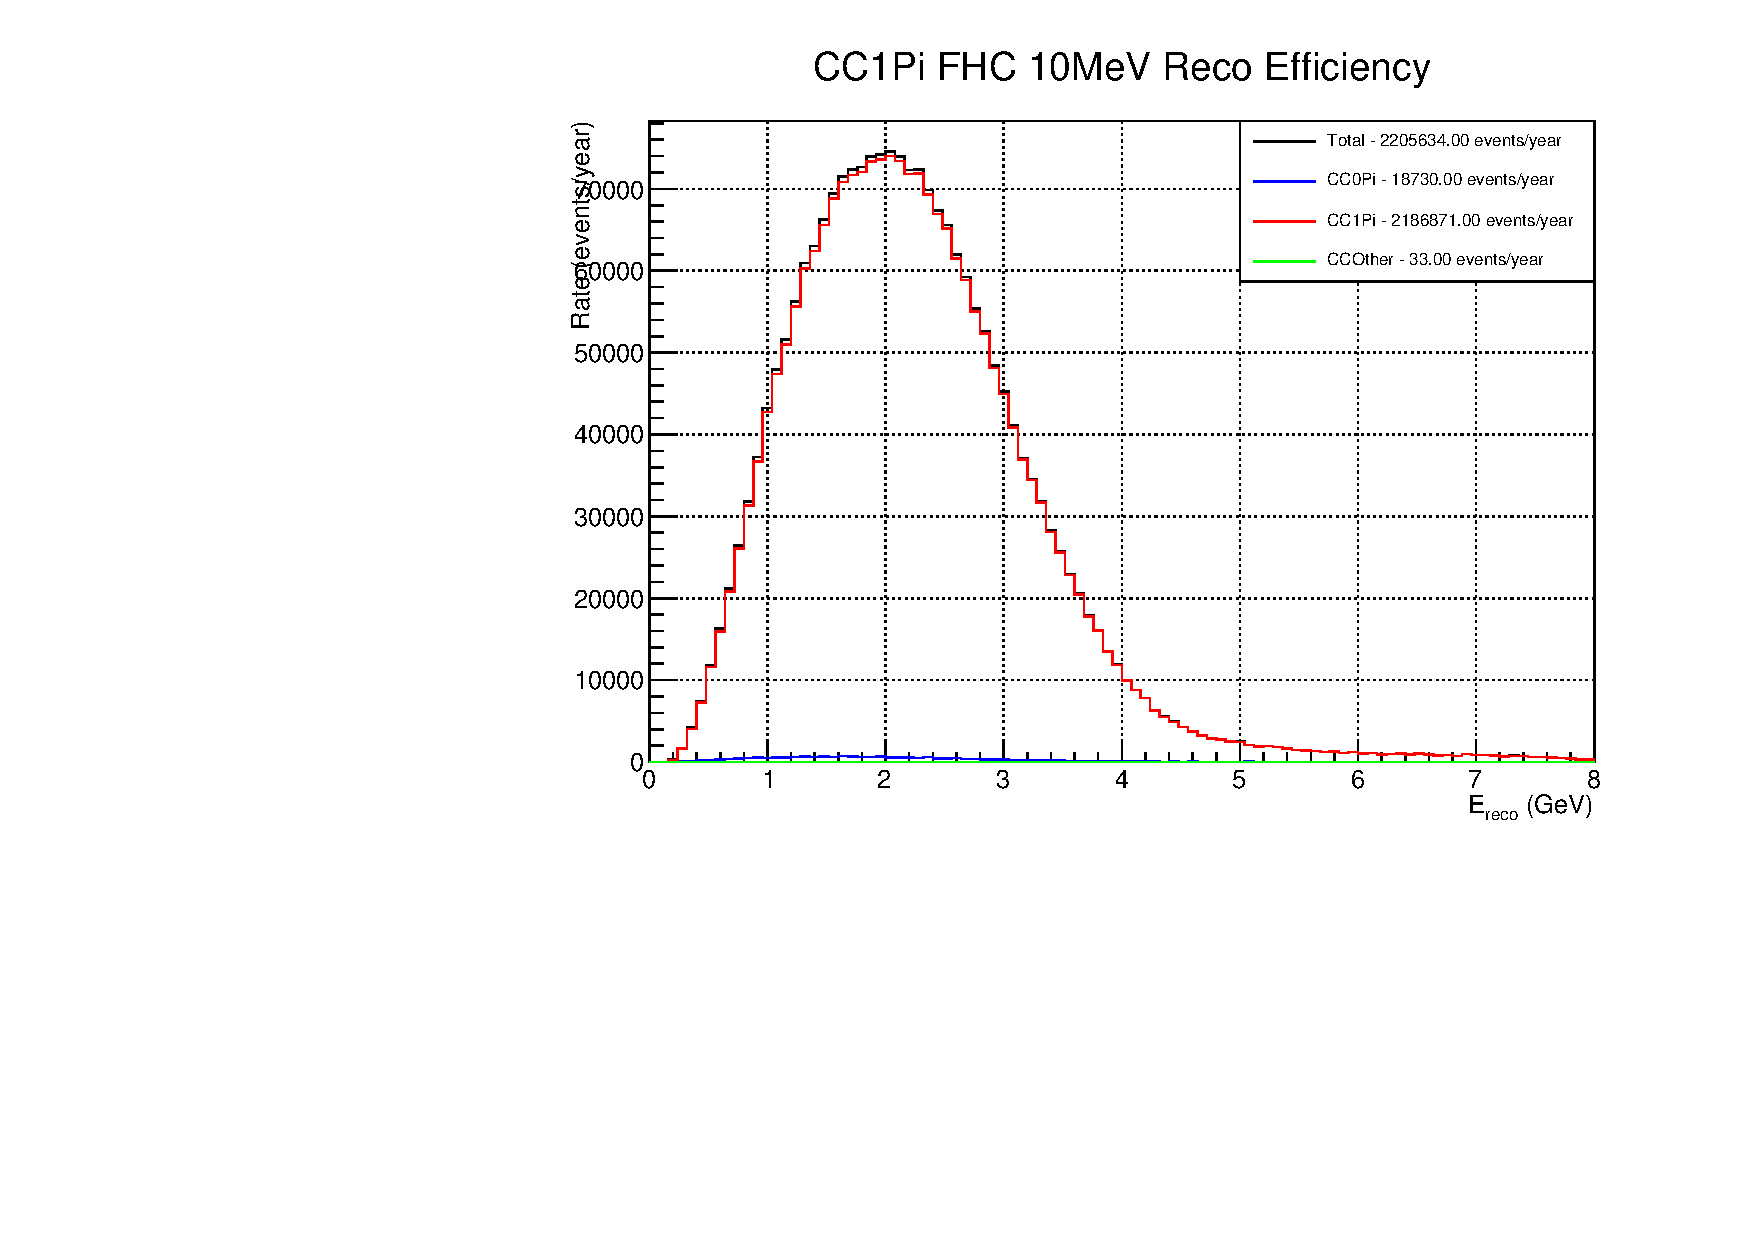
\includegraphics[width=0.245\textwidth]{plots/efficiency/CC1Pi_FHC_10MeV.pdf} 
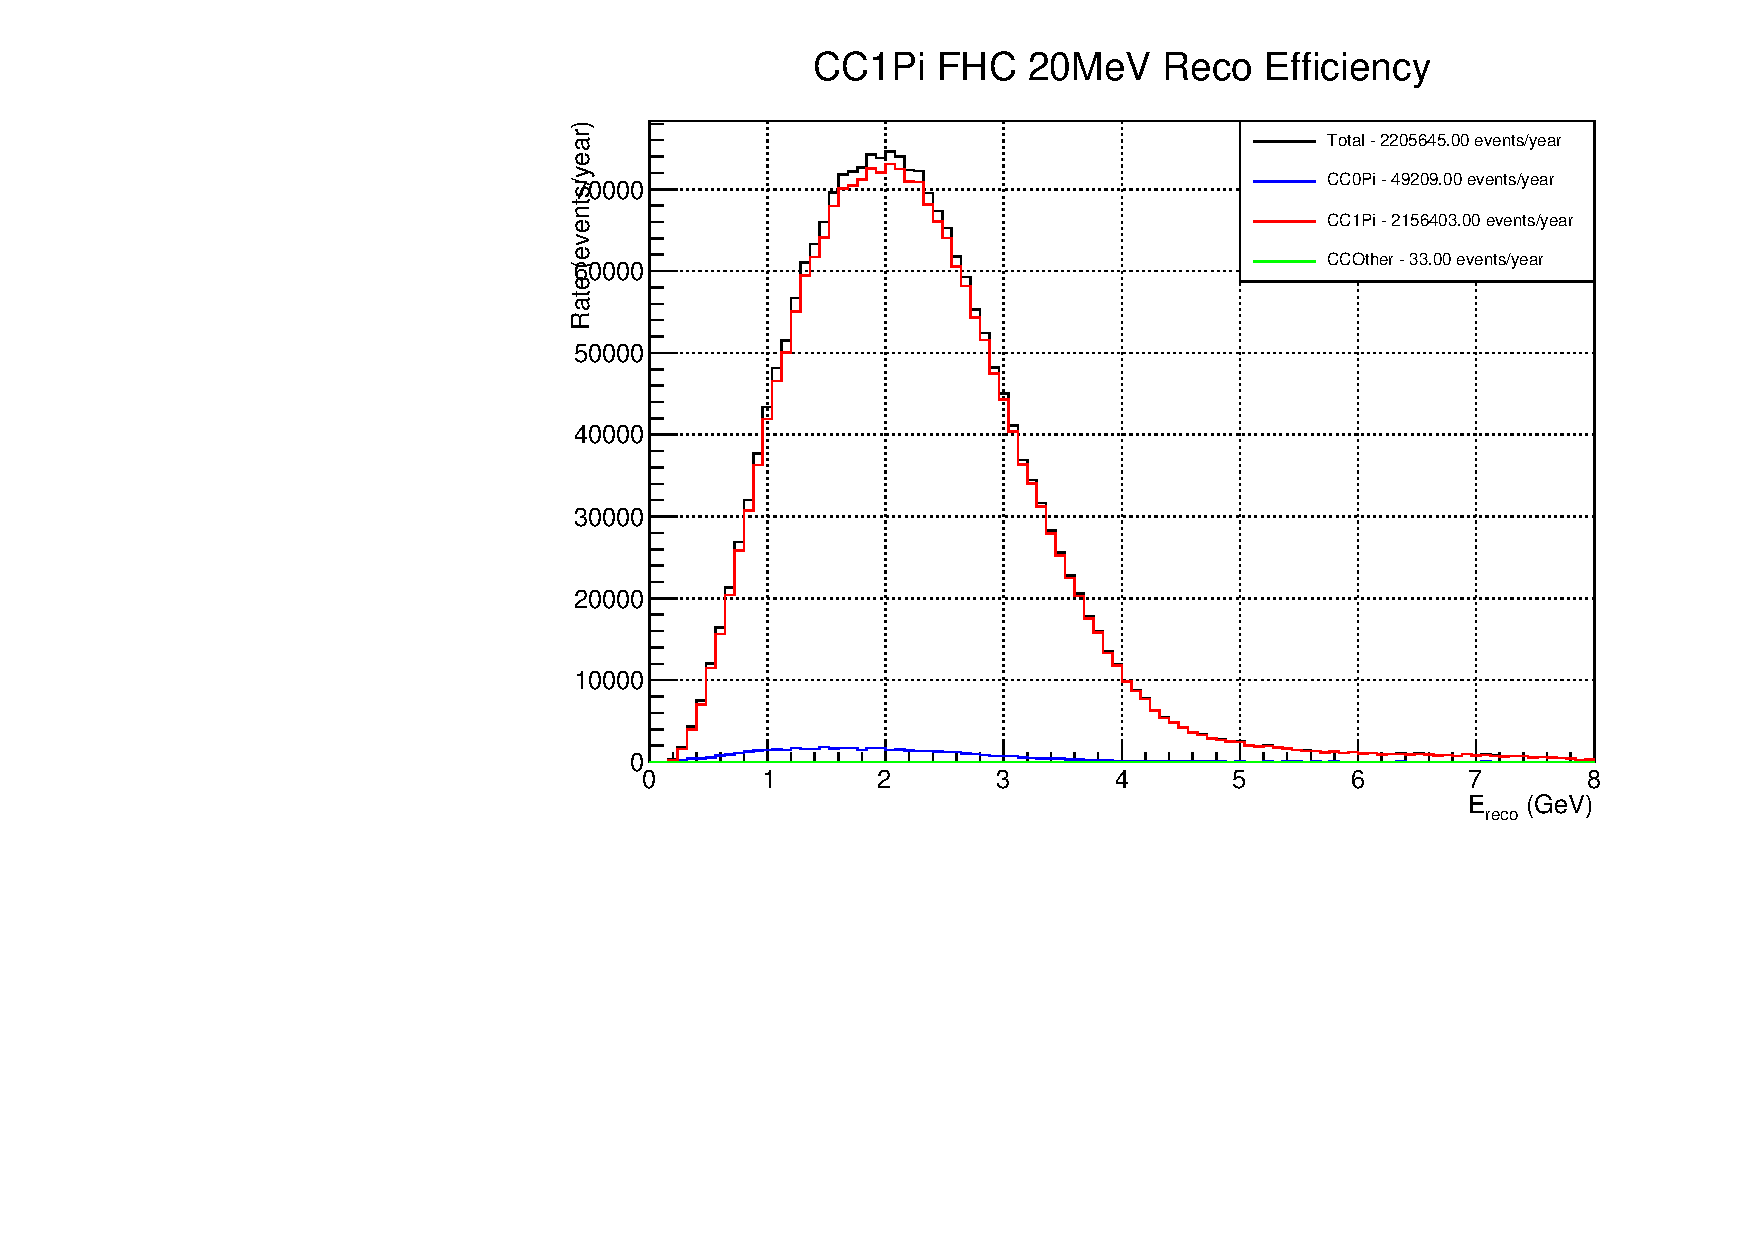
\includegraphics[width=0.245\textwidth]{plots/efficiency/CC1Pi_FHC_20MeV.pdf}
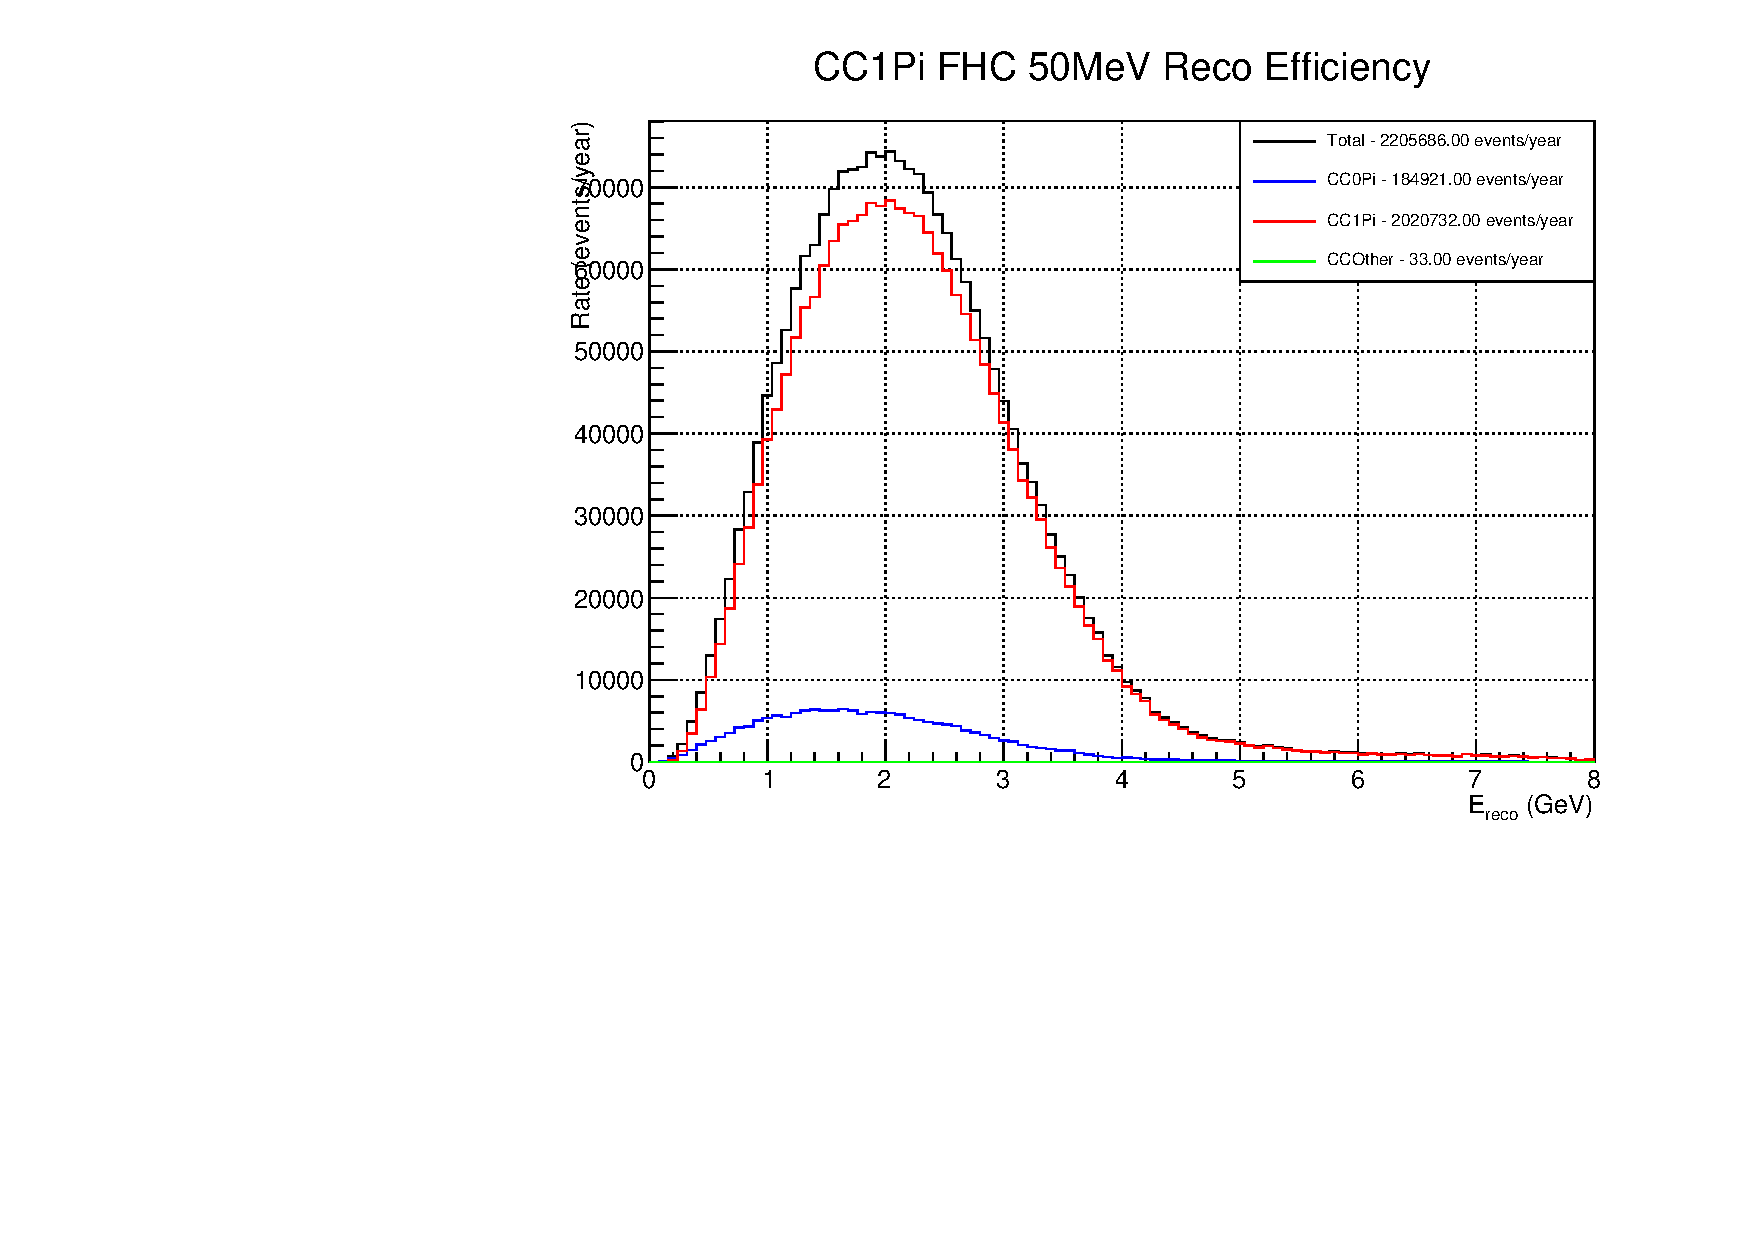
\includegraphics[width=0.245\textwidth]{plots/efficiency/CC1Pi_FHC_50MeV.pdf}

\end{center}

\subsubsection{CCOther}

True CCOther events can be reconstructed as CC1Pi or CC0Pi depending upon how many pions are beneath the tracking threshold.

\begin{center}

\includegraphics[width=0.245\textwidth]{plots/efficiency/CCOther_FHC_No_Threshold.pdf}
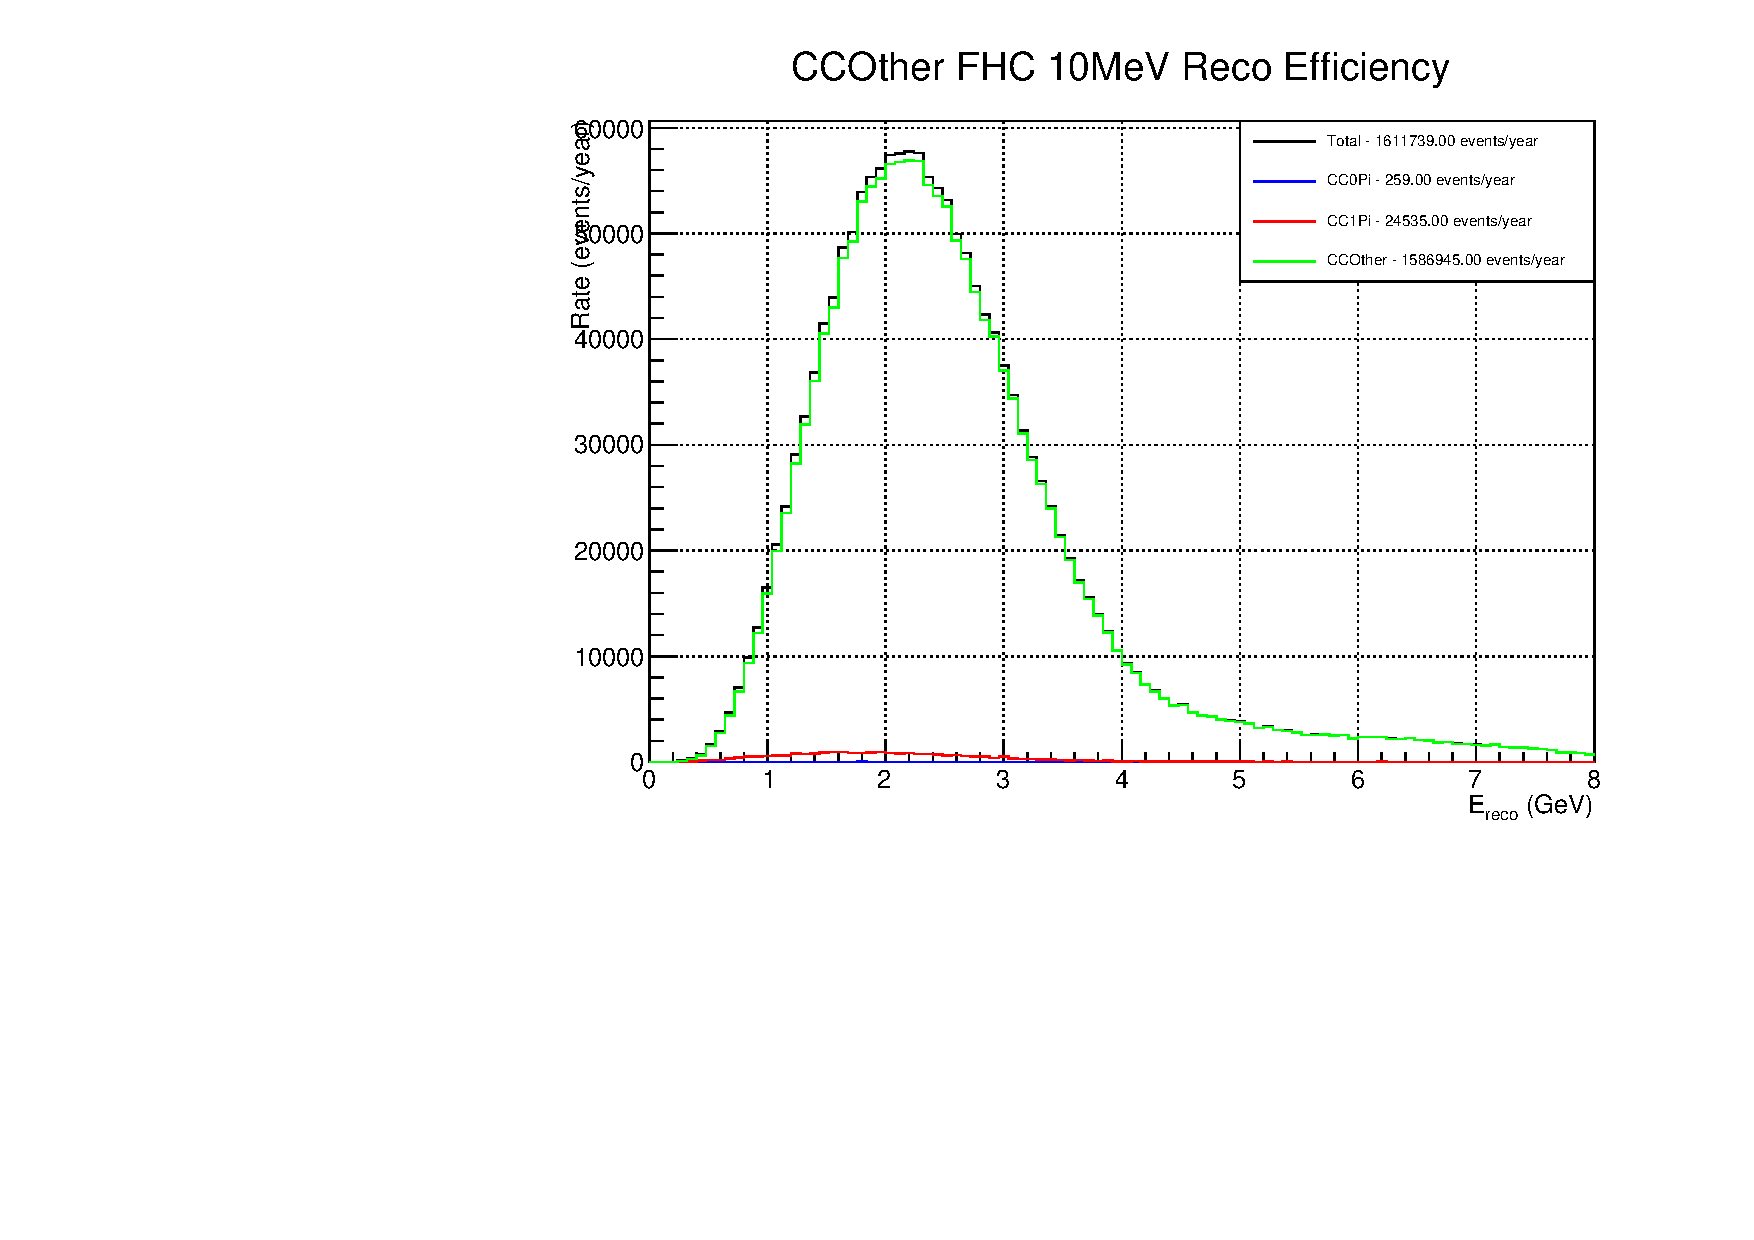
\includegraphics[width=0.245\textwidth]{plots/efficiency/CCOther_FHC_10MeV.pdf} 
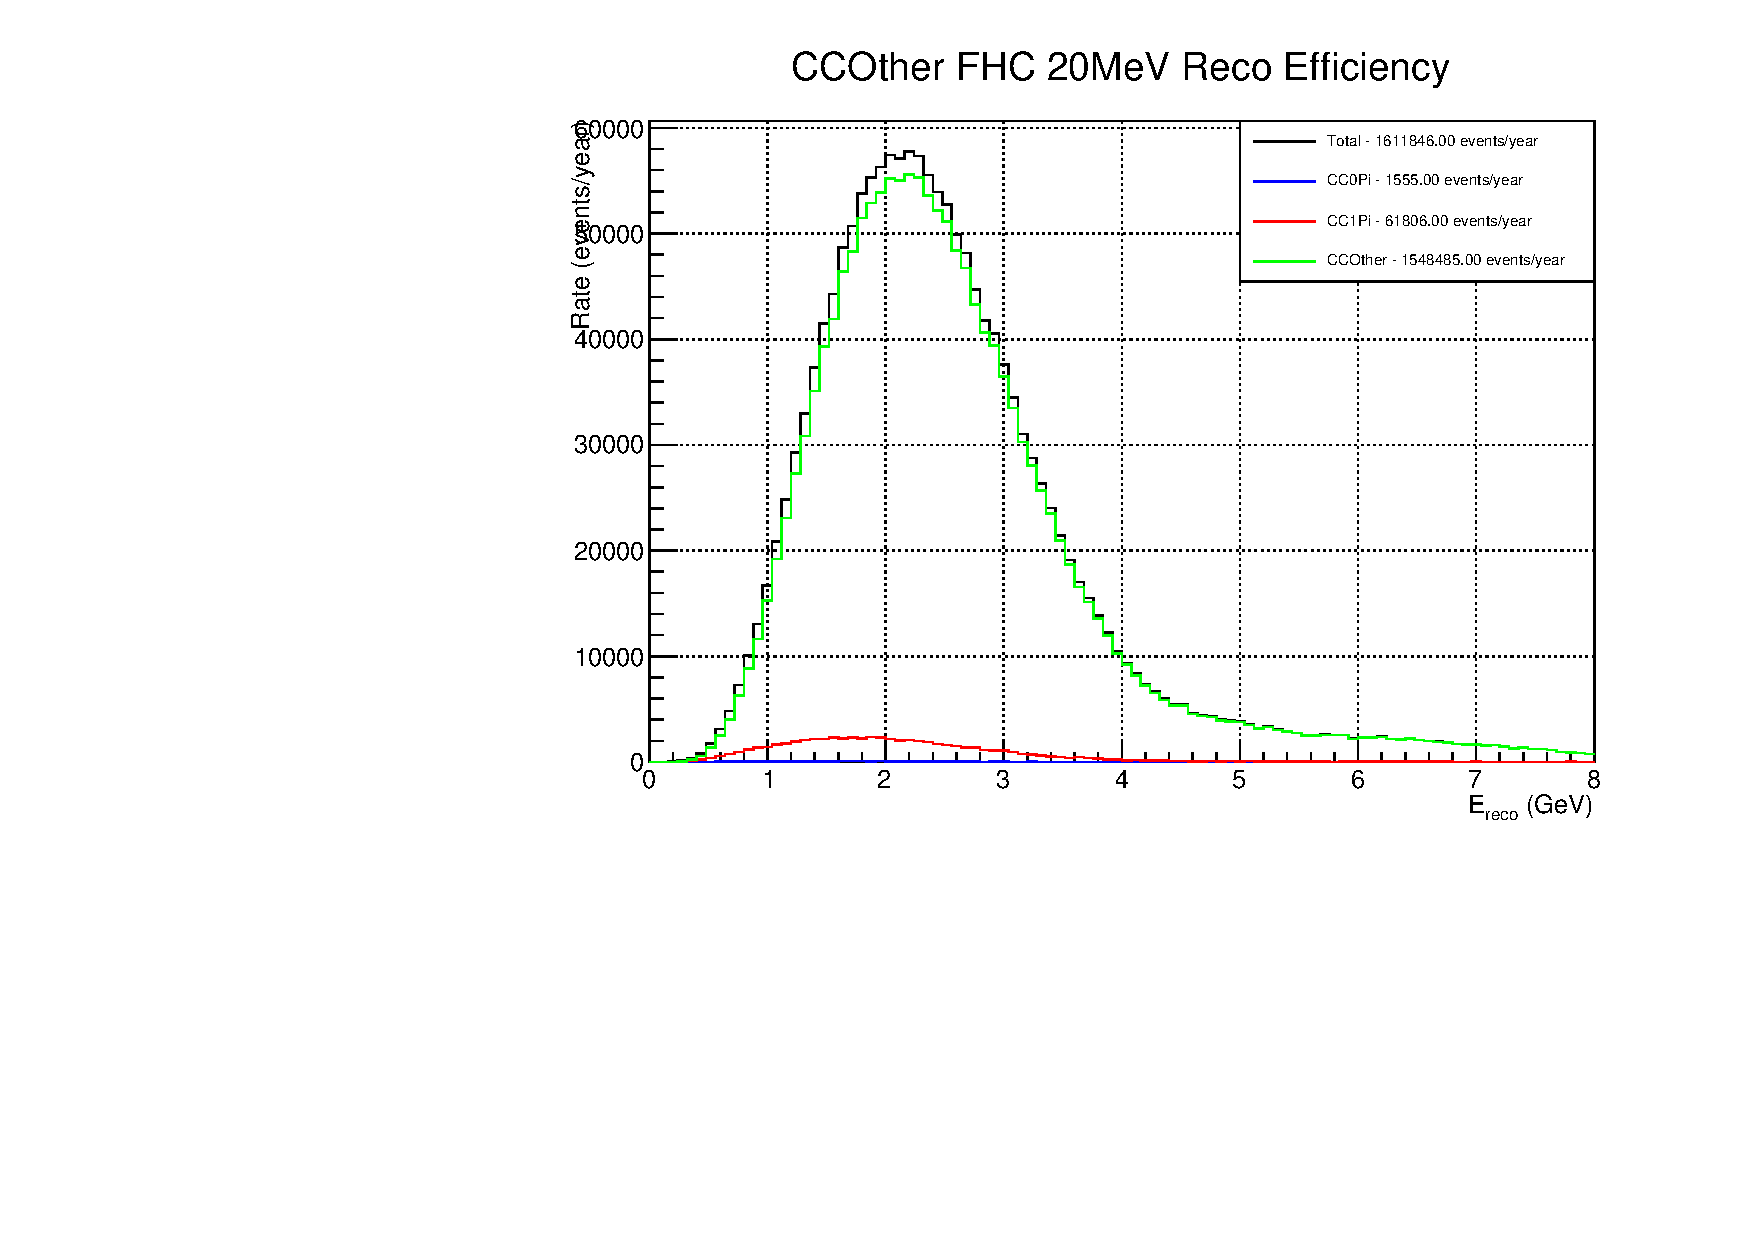
\includegraphics[width=0.245\textwidth]{plots/efficiency/CCOther_FHC_20MeV.pdf}
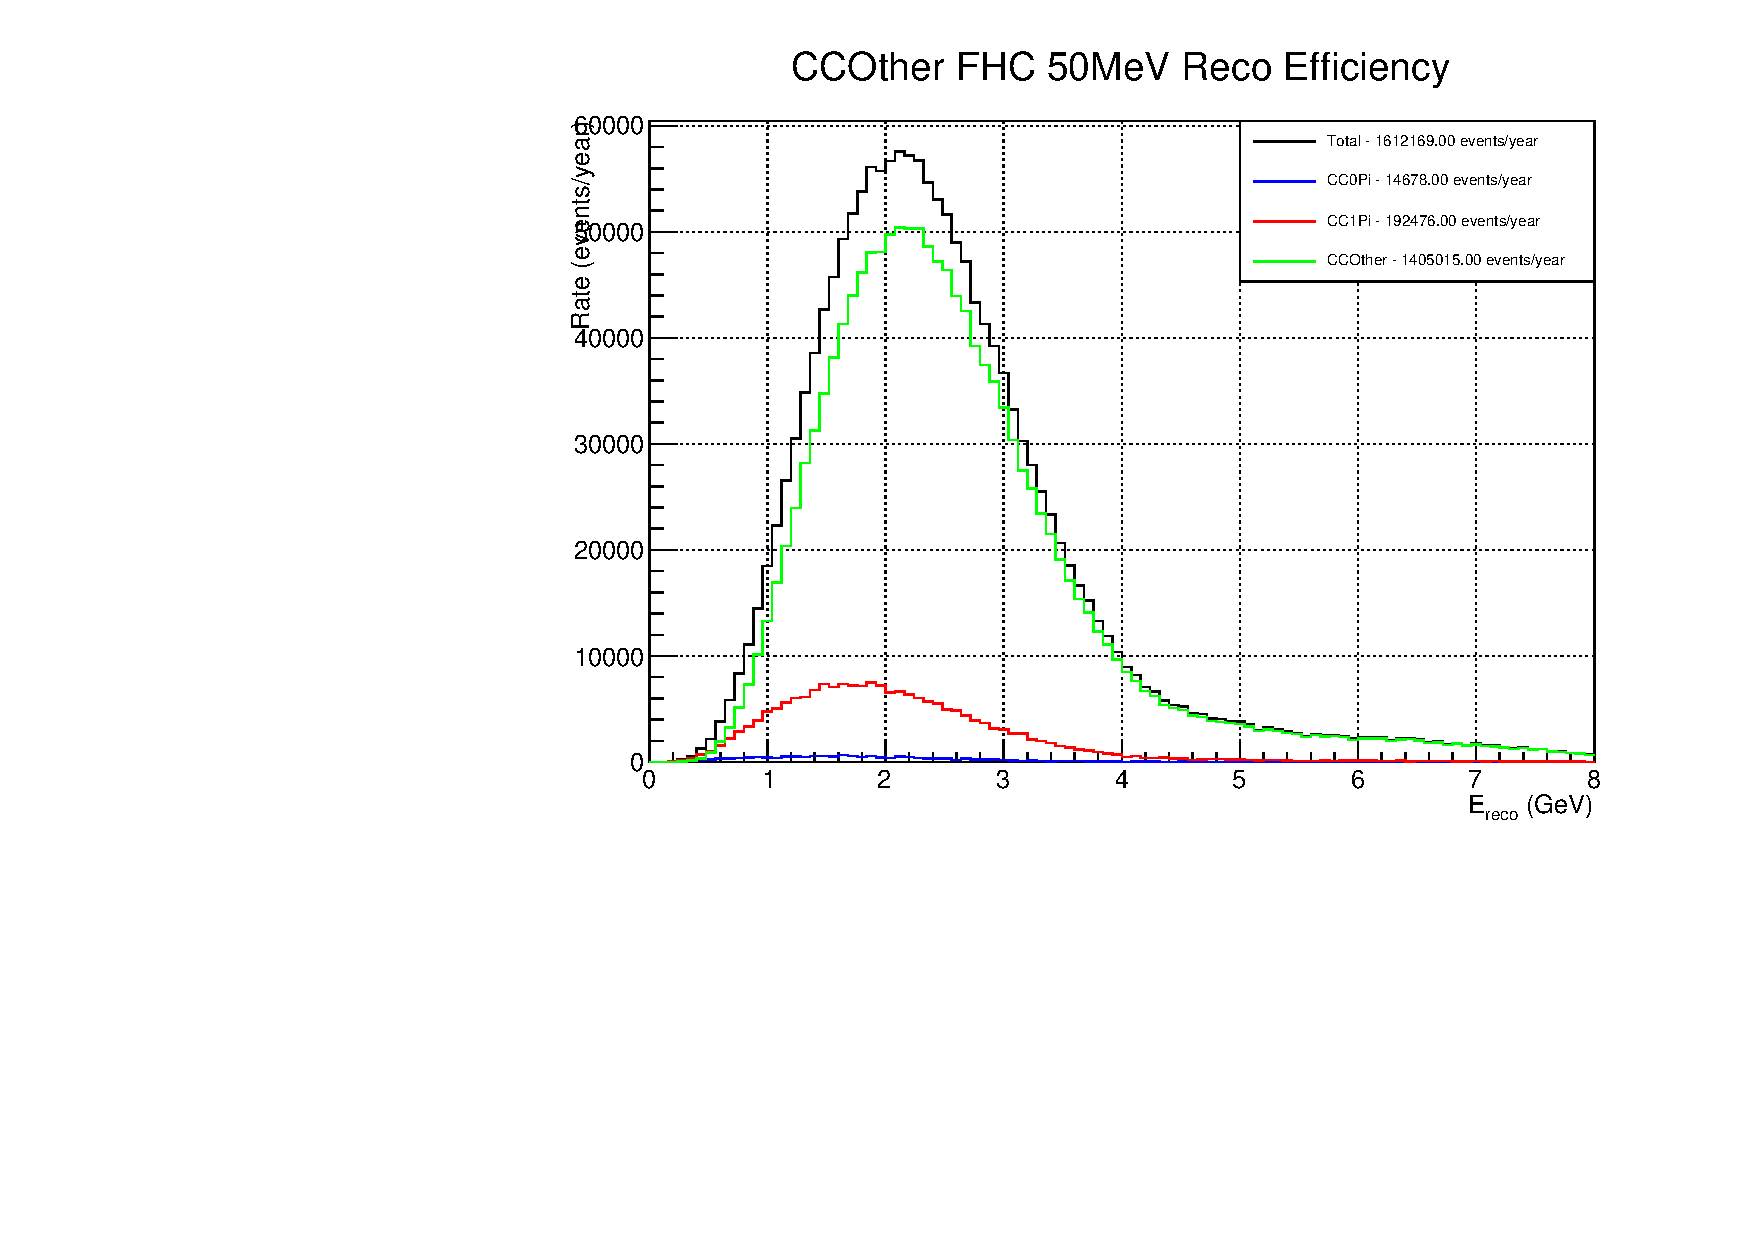
\includegraphics[width=0.245\textwidth]{plots/efficiency/CCOther_FHC_50MeV.pdf}

\end{center}


\subsection{RHC}

\subsubsection{CC0Pi}

\begin{center}

\includegraphics[width=0.245\textwidth]{plots/efficiency/CC0Pi_RHC_No_Threshold.pdf}
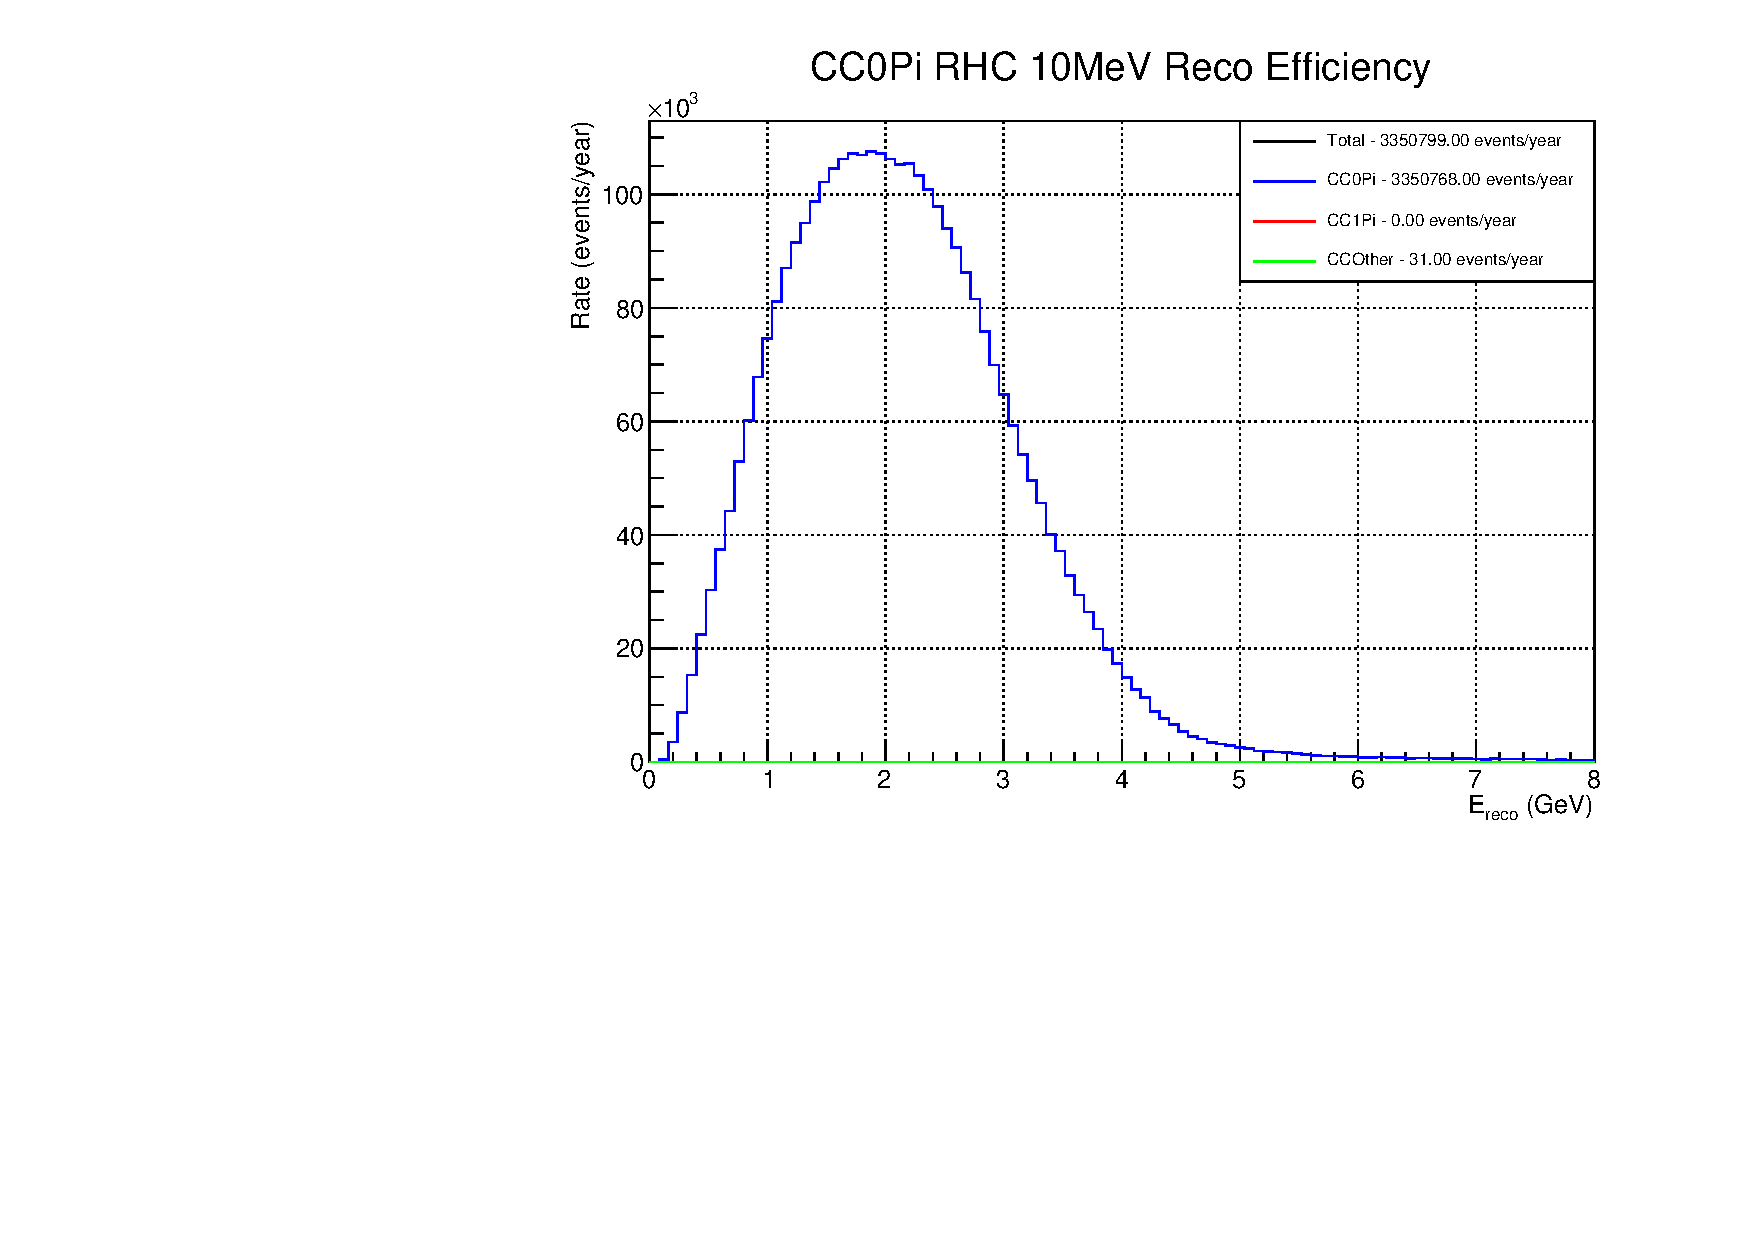
\includegraphics[width=0.245\textwidth]{plots/efficiency/CC0Pi_RHC_10MeV.pdf} 
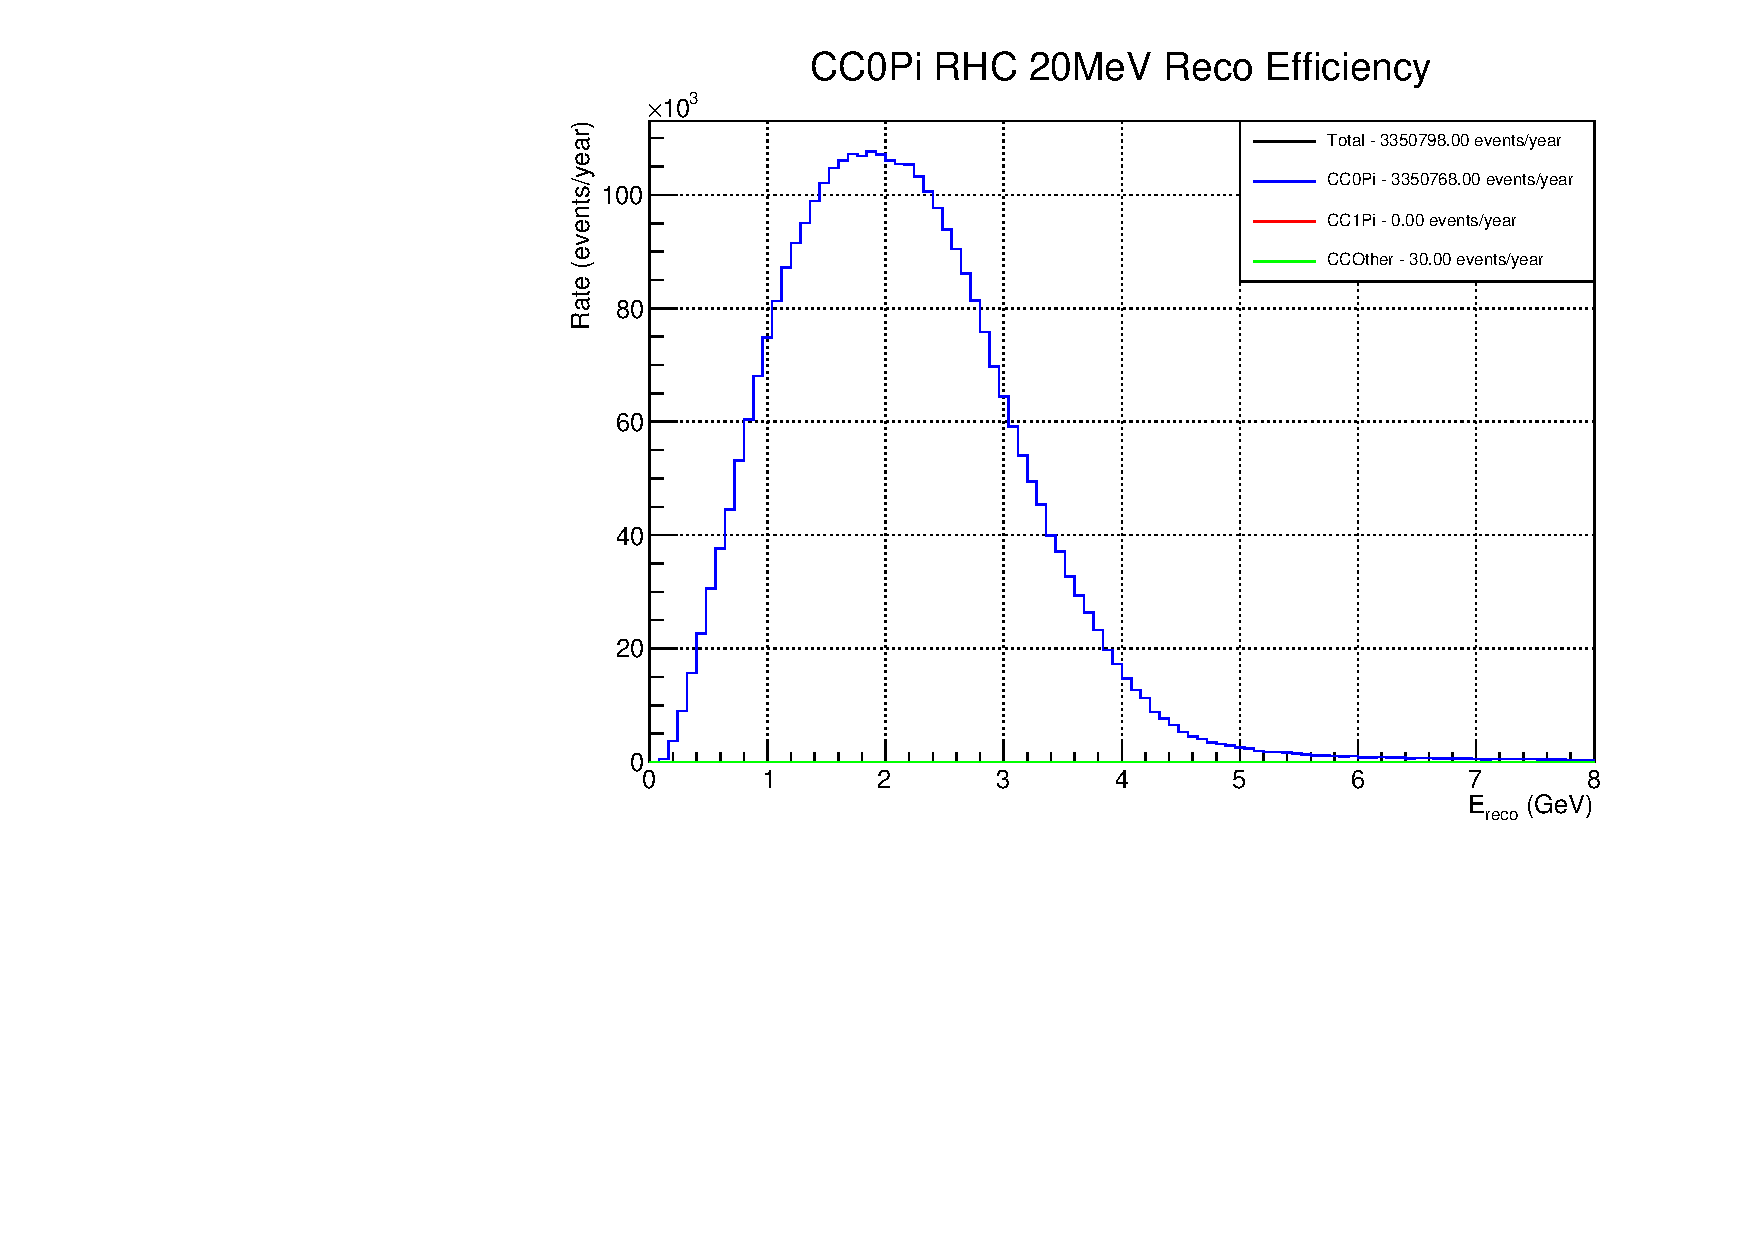
\includegraphics[width=0.245\textwidth]{plots/efficiency/CC0Pi_RHC_20MeV.pdf}
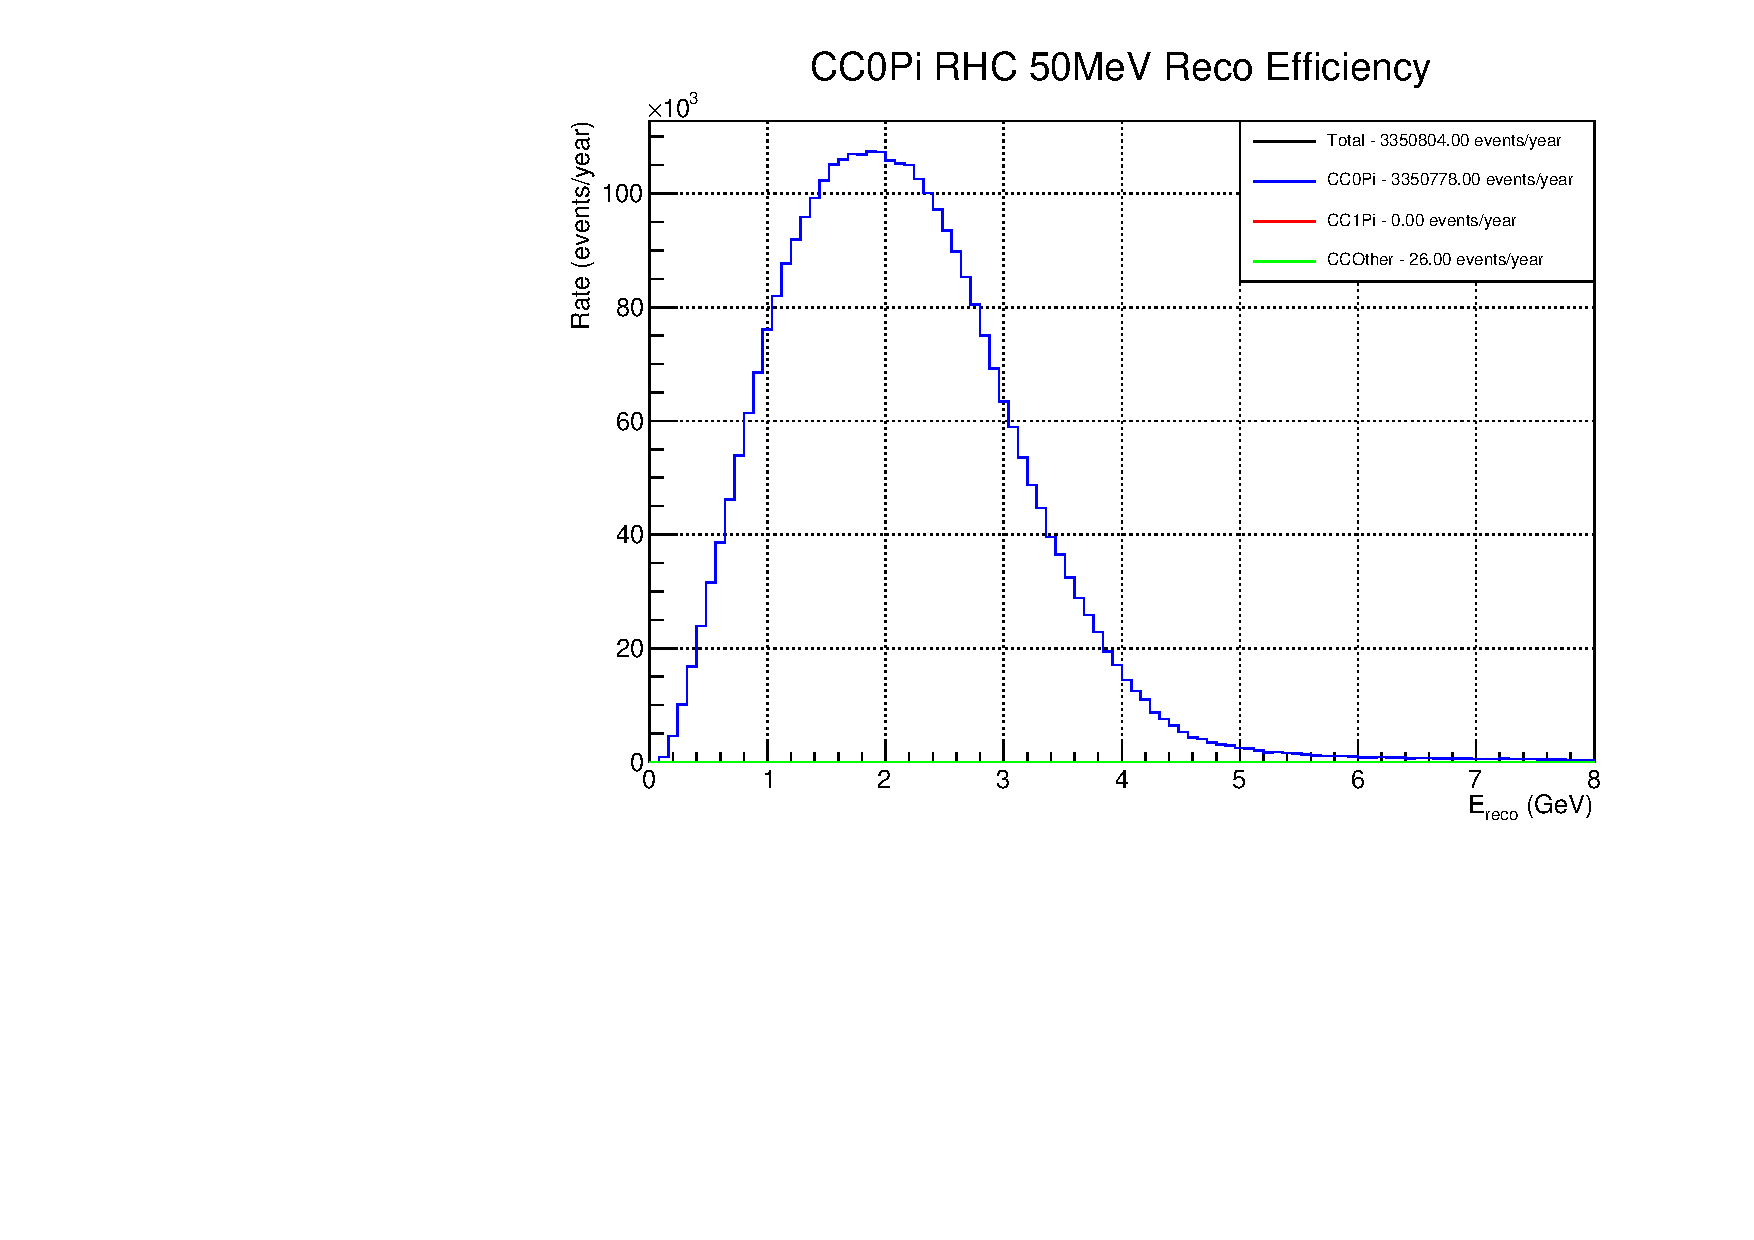
\includegraphics[width=0.245\textwidth]{plots/efficiency/CC0Pi_RHC_50MeV.pdf}

\end{center}

\subsubsection{CC1Pi}

\begin{center}

\includegraphics[width=0.245\textwidth]{plots/efficiency/CC1Pi_RHC_No_Threshold.pdf}
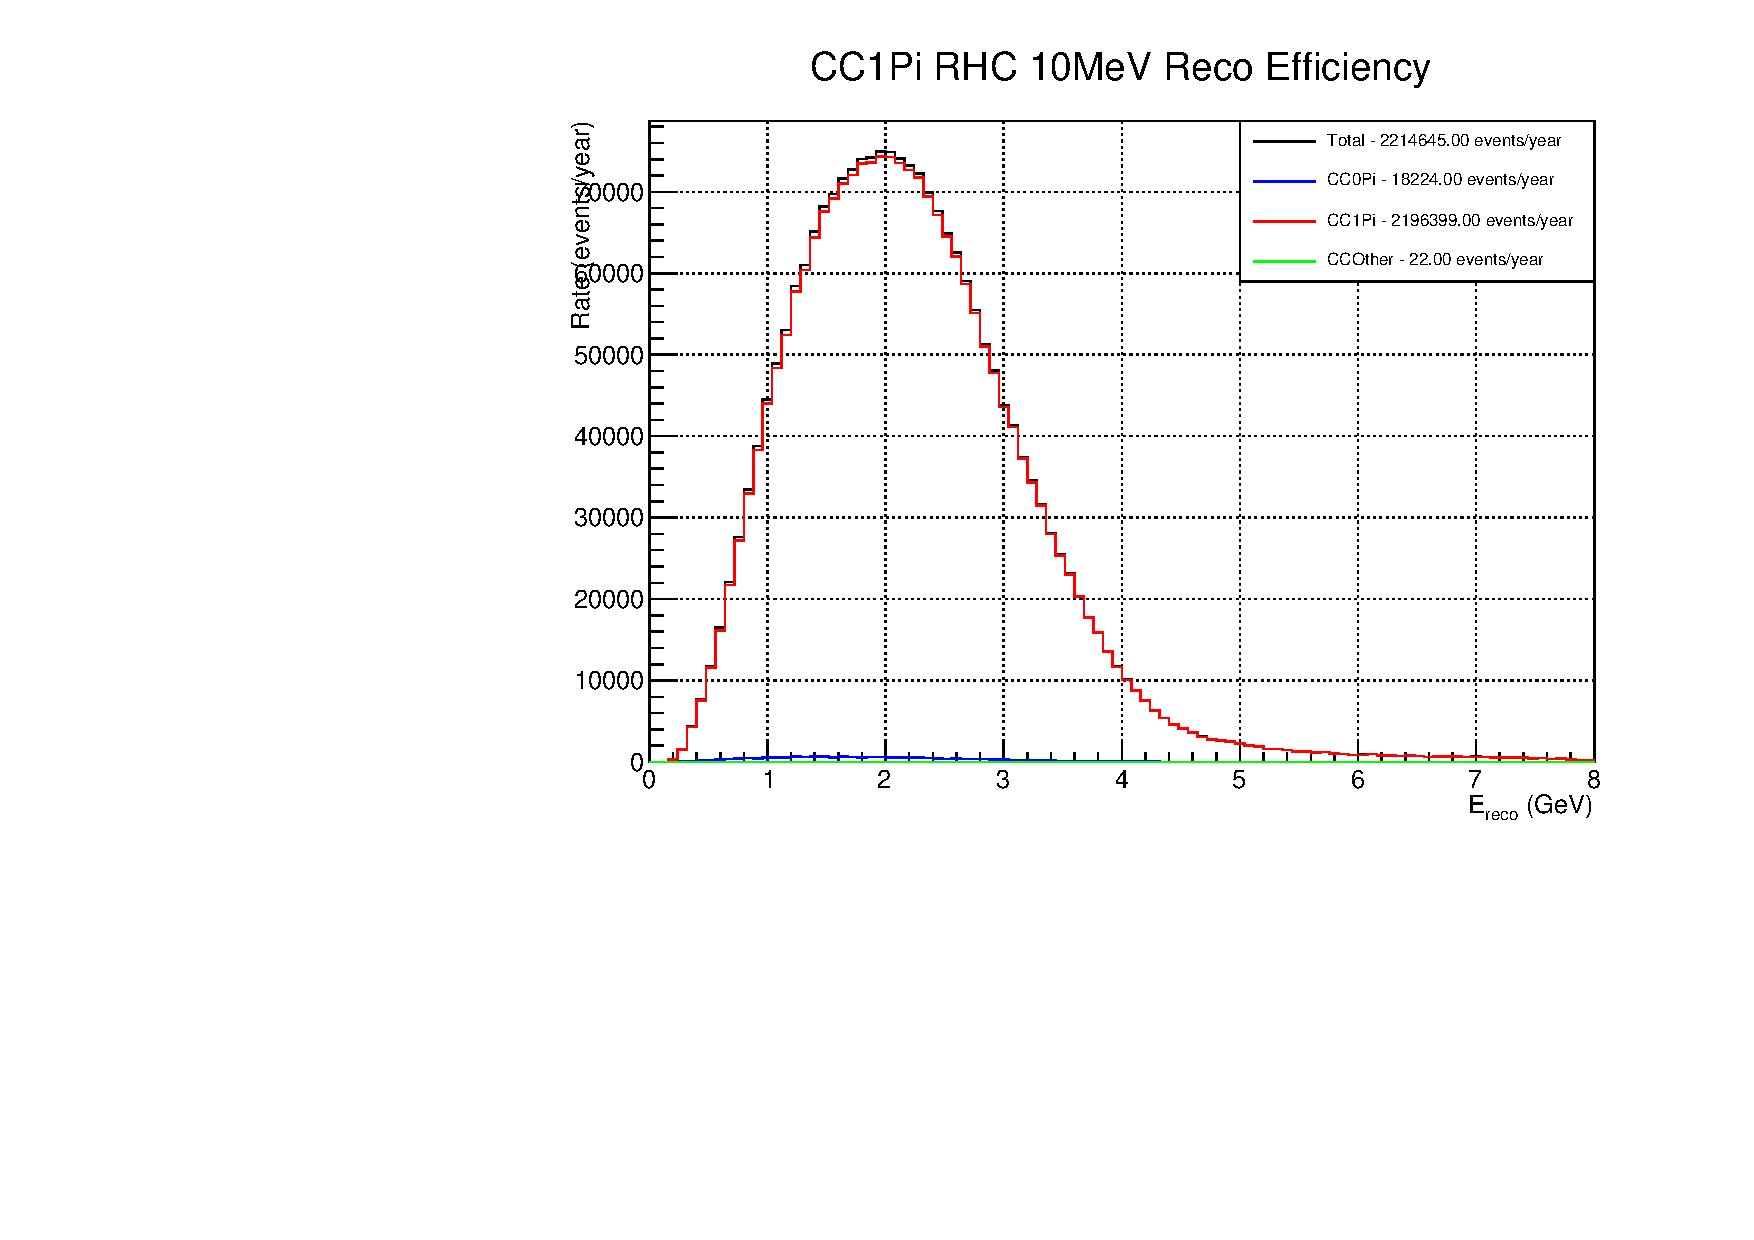
\includegraphics[width=0.245\textwidth]{plots/efficiency/CC1Pi_RHC_10MeV.pdf} 
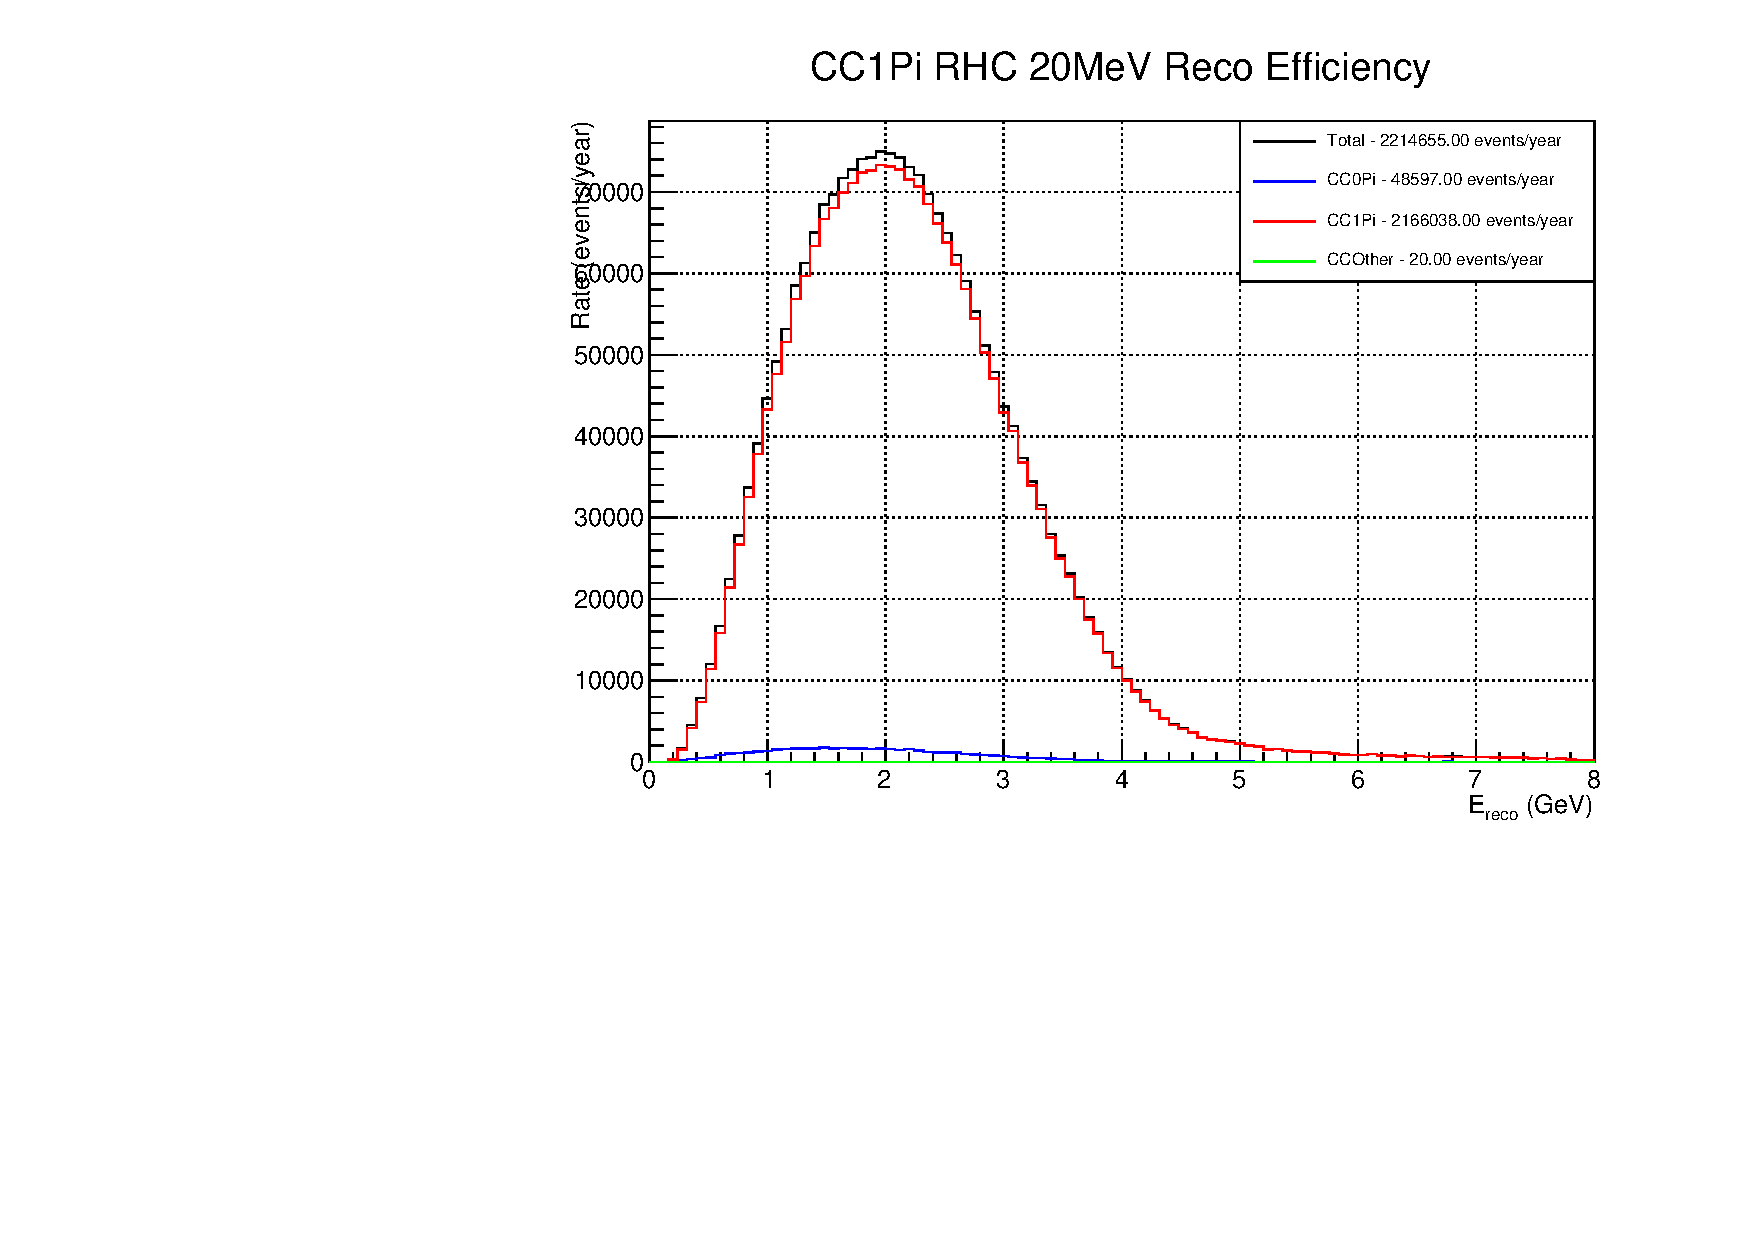
\includegraphics[width=0.245\textwidth]{plots/efficiency/CC1Pi_RHC_20MeV.pdf}
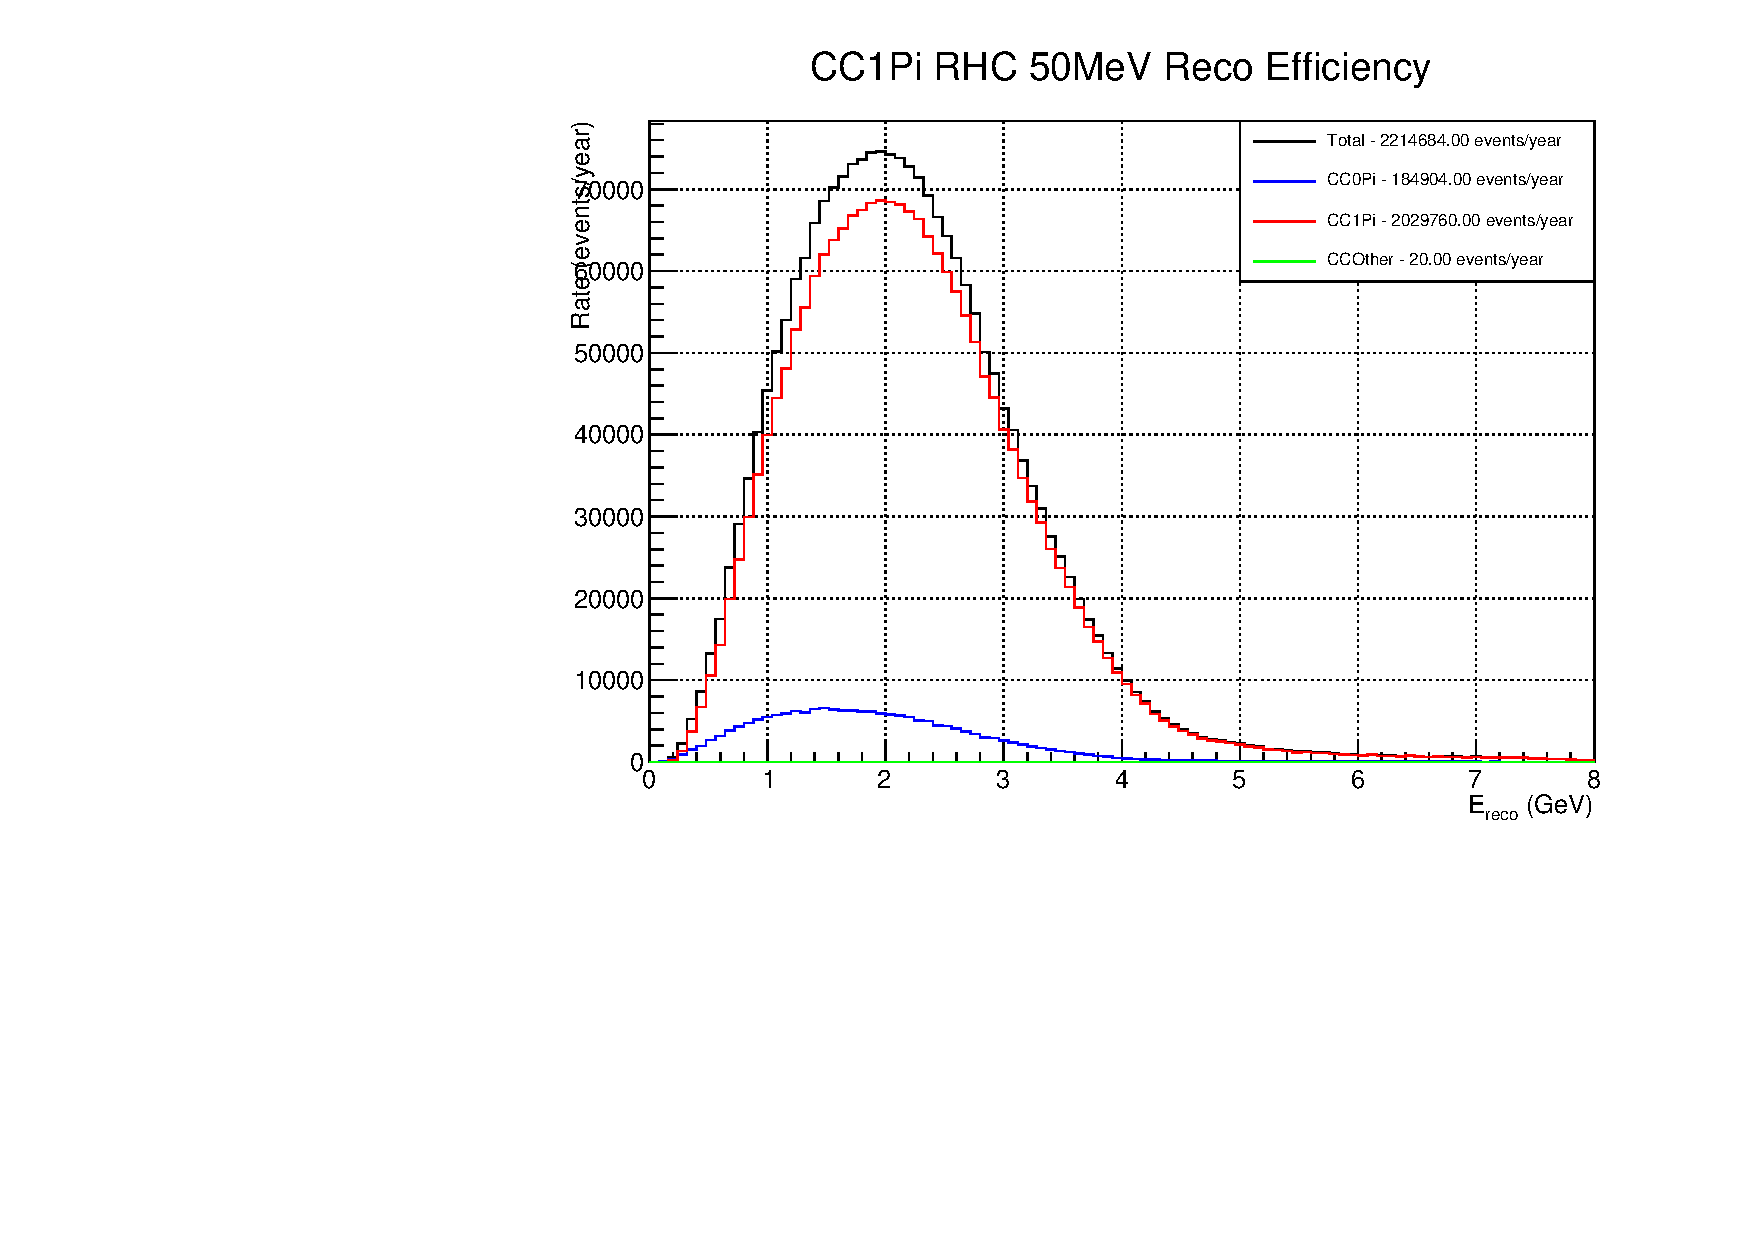
\includegraphics[width=0.245\textwidth]{plots/efficiency/CC1Pi_RHC_50MeV.pdf}

\end{center}

\subsubsection{CCOther}

\begin{center}

\includegraphics[width=0.245\textwidth]{plots/efficiency/CCOther_RHC_No_Threshold.pdf}
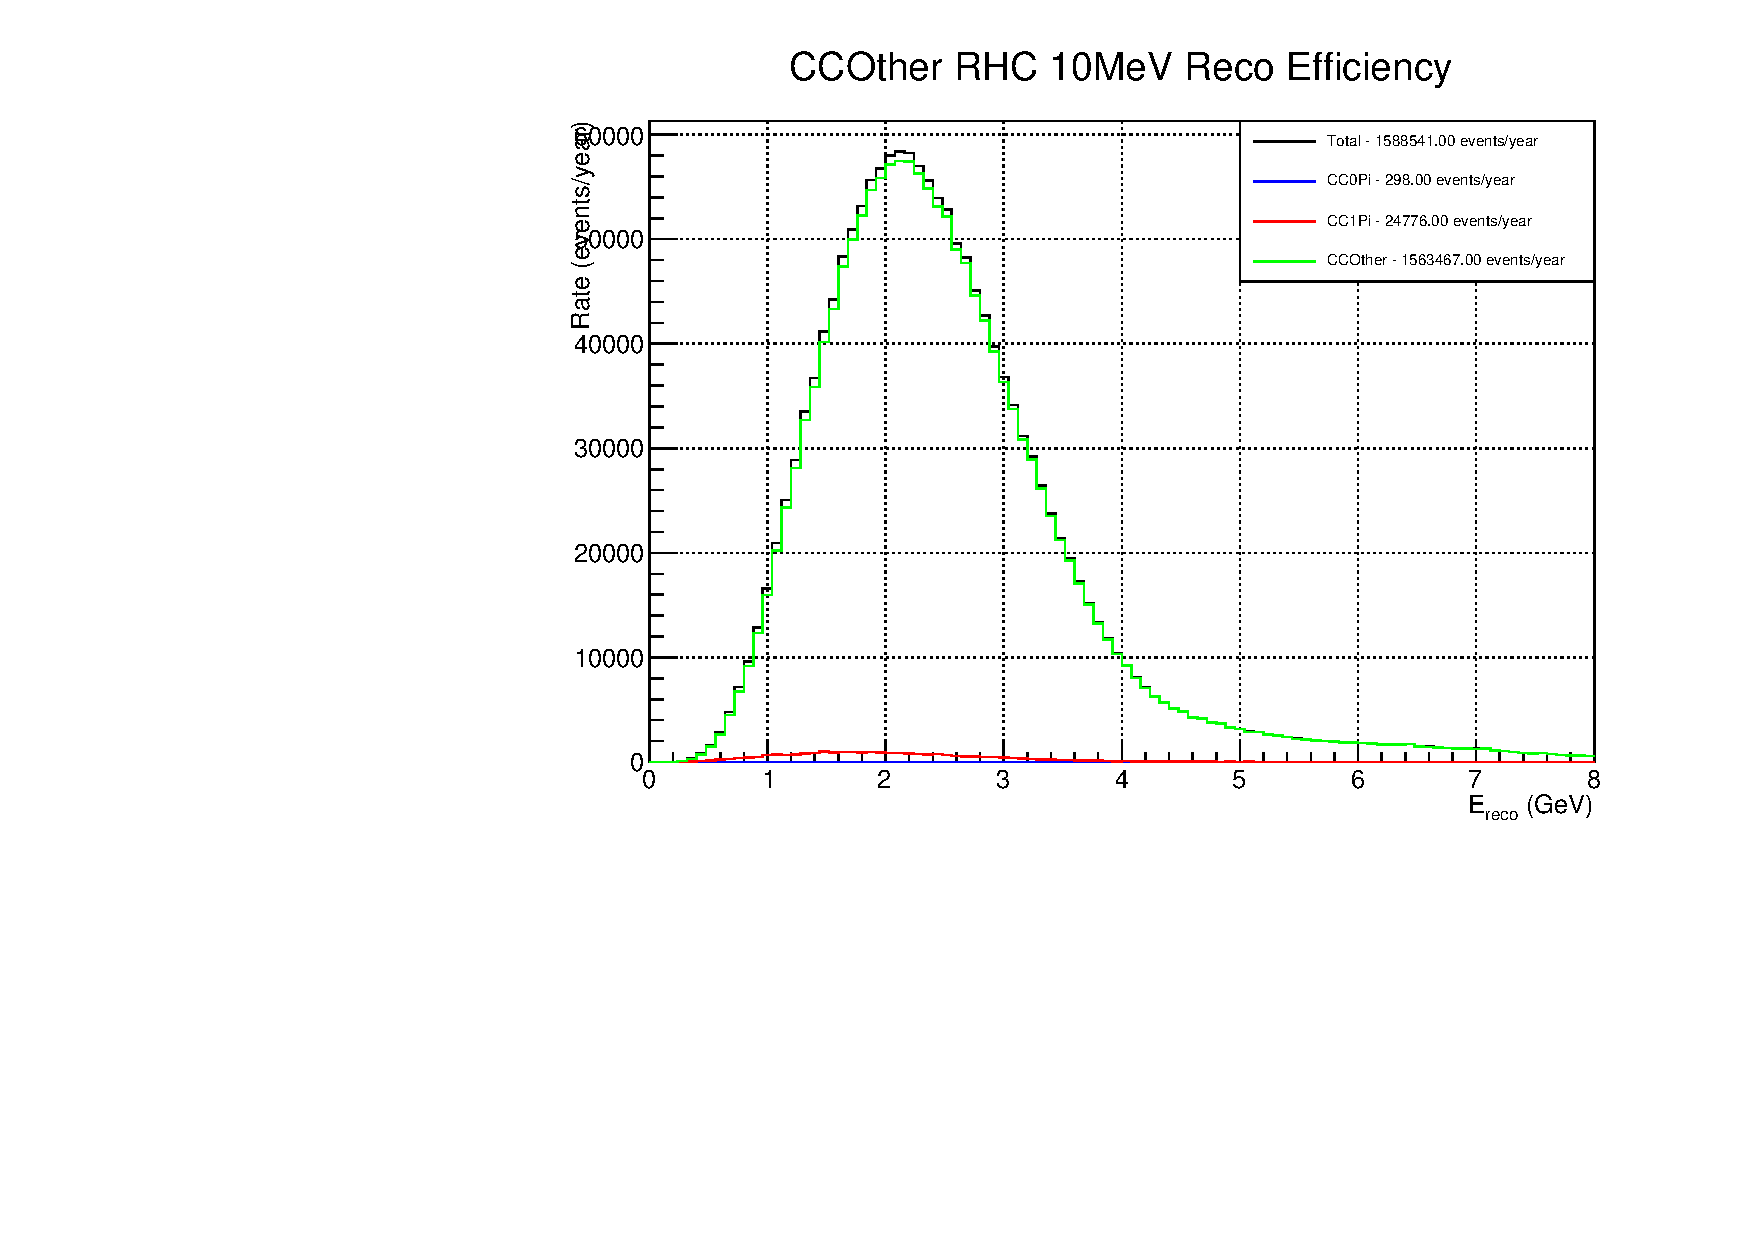
\includegraphics[width=0.245\textwidth]{plots/efficiency/CCOther_RHC_10MeV.pdf} 
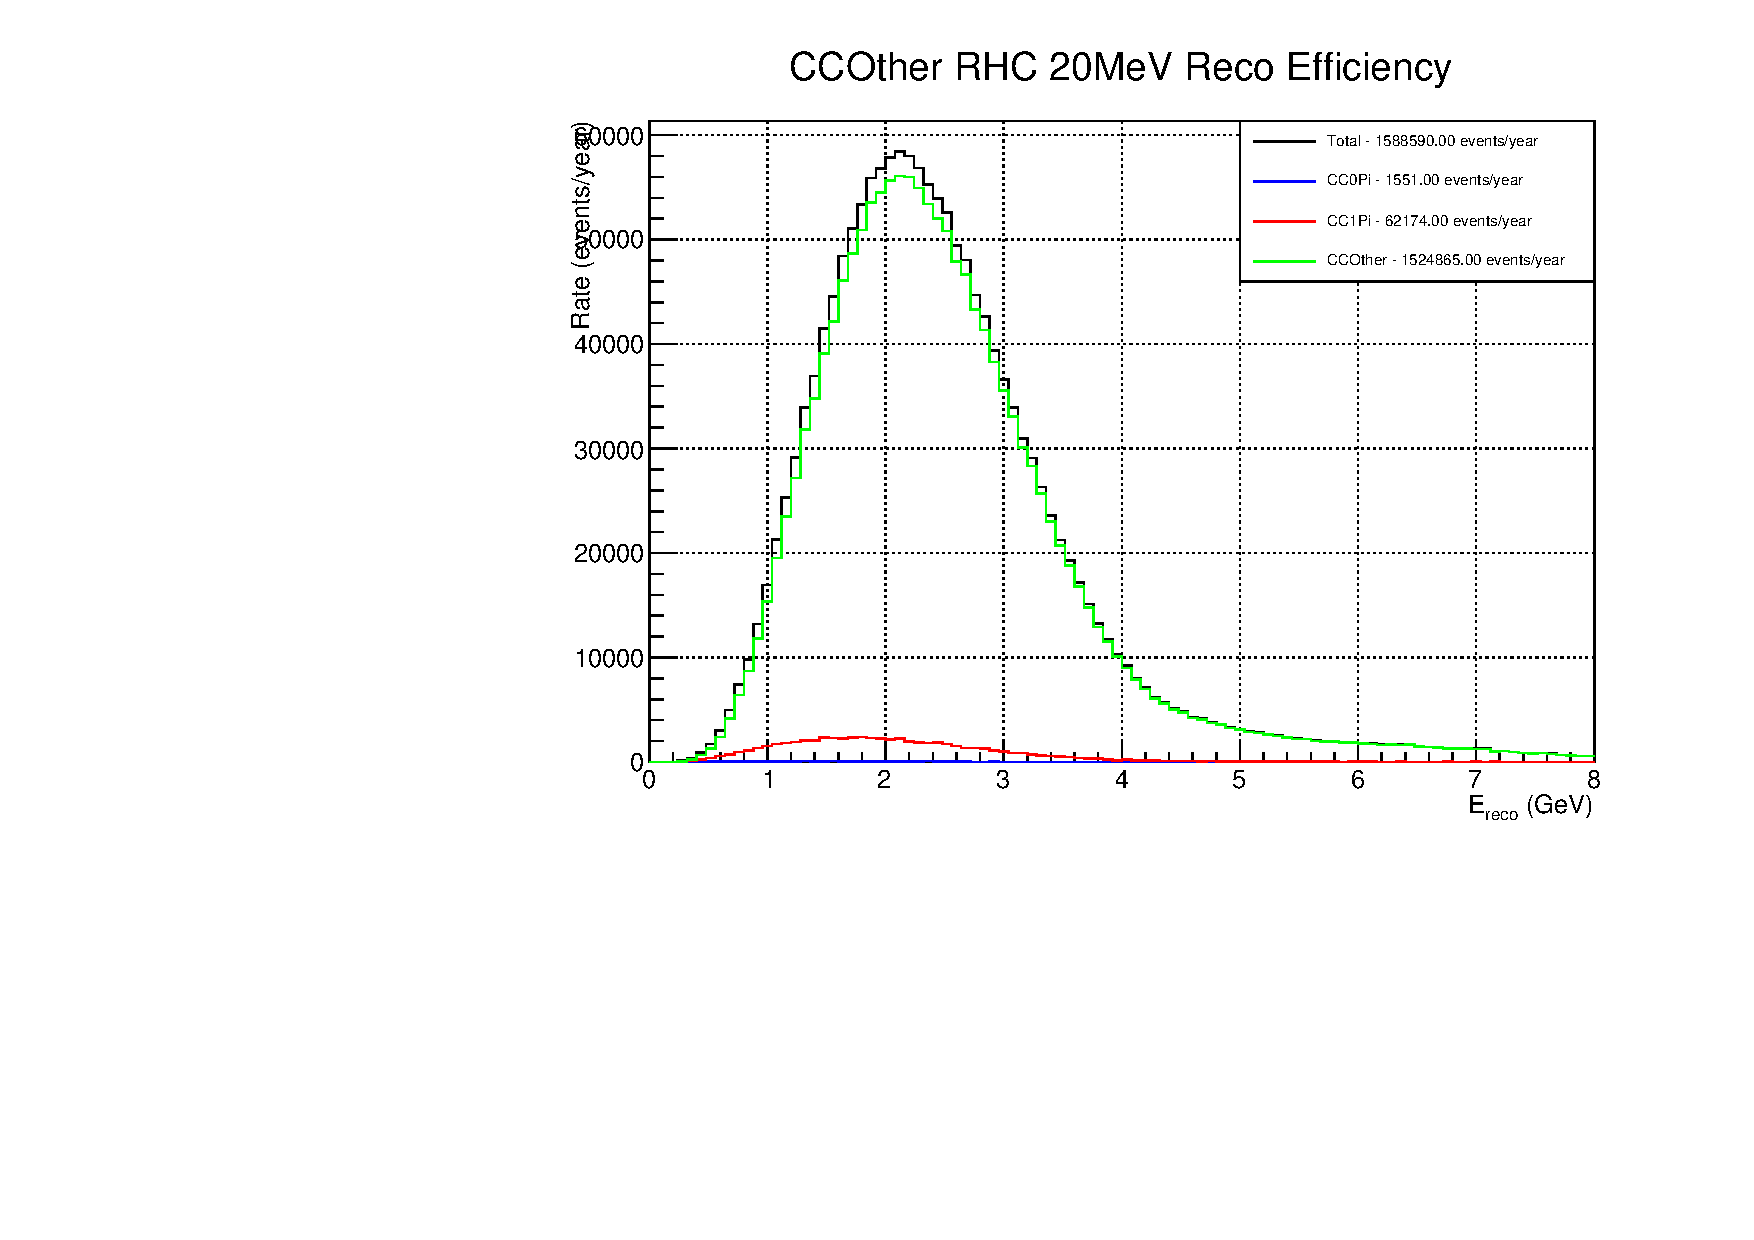
\includegraphics[width=0.245\textwidth]{plots/efficiency/CCOther_RHC_20MeV.pdf}
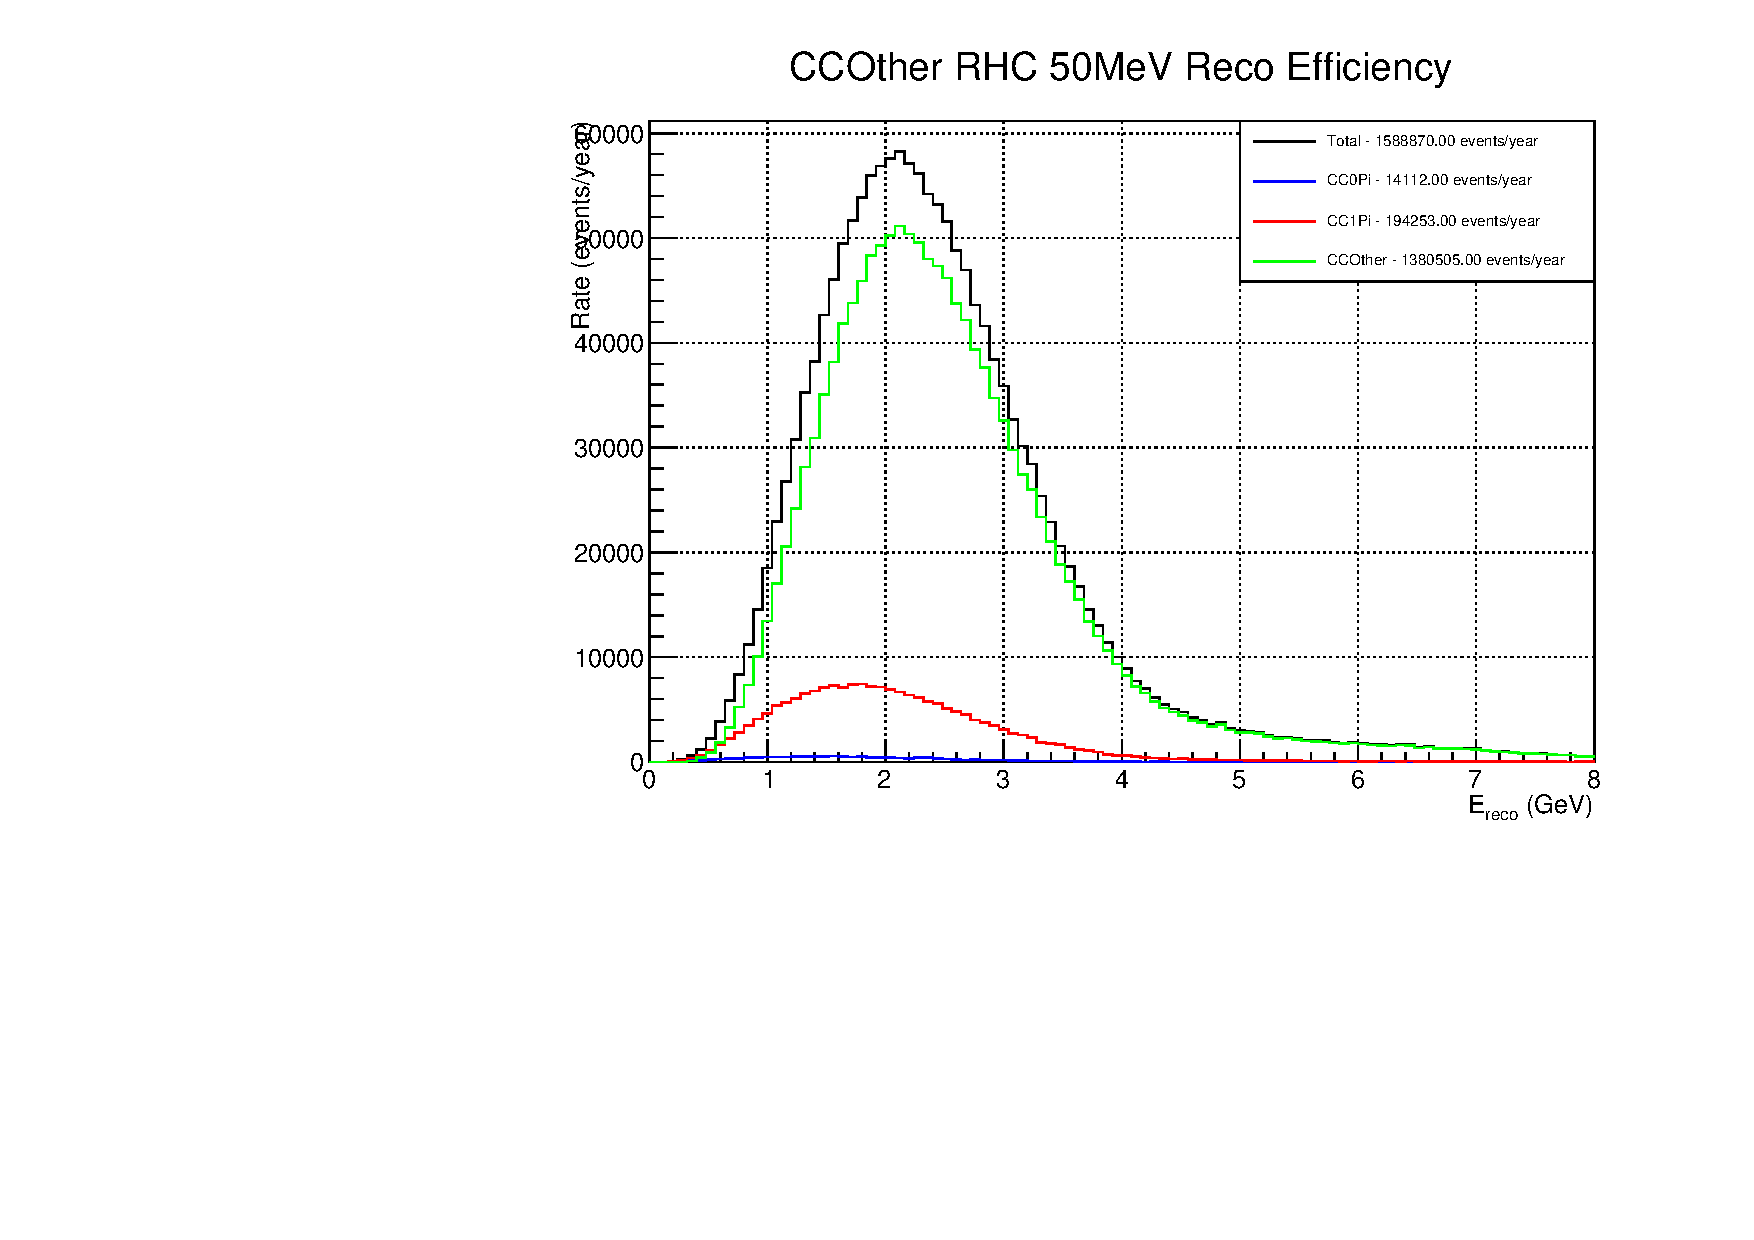
\includegraphics[width=0.245\textwidth]{plots/efficiency/CCOther_RHC_50MeV.pdf}

\end{center}
